\documentclass[11pt,a4paper]{article}

\usepackage[utf8]{inputenc}
\usepackage[english]{babel}
\usepackage[left=2cm,right=2cm,top=2cm,bottom=2cm]{geometry}

\usepackage{csquotes}
\usepackage{graphicx}
\graphicspath{ {./figs} }

\usepackage{caption}
\usepackage{subcaption}

\usepackage{amsmath}
\usepackage{amssymb}
\usepackage{amsthm}

\usepackage{mathrsfs}
\usepackage{mathtools}

\usepackage{color}
\usepackage{epsfig}
\usepackage{array}
\usepackage{multicol}
\usepackage{tikz}
\usepackage{listings}
\usepackage{minted}
\usepackage{mdframed}

\setlength{\parindent}{0em}
\setlength{\parskip}{0.5em}
% \textwidth 6.5in
% \textheight 9.in
% \oddsidemargin 0in
% \headheight 0in


\newtheorem{theorem}{Theorem}[section]

\definecolor{codegreen}{rgb}{0,0.6,0}
\definecolor{codegray}{rgb}{0.5,0.5,0.5}
\definecolor{backcolour}{rgb}{0.95,0.95,0.95}

\usepackage[hidelinks]{hyperref}
\hypersetup{
    colorlinks=false, %set true if you want colored links
    linktoc=all,      %set to all if you want both sections & subsections linked
}


\lstset{ %
  language=python,                % choose the language of the code
  basicstyle=\footnotesize,       % the size of the fonts that are used for the code
  numbers=left,                   % where to put the line-numbers
  numberstyle=\footnotesize,      % the size of the fonts that are used for the line-numbers
  stepnumber=1,                   % the step between two line-numbers. If it is 1 each line will be numbered
  numbersep=5pt,                  % how far the line-numbers are from the code
  backgroundcolor=\color{white},  % choose the background color. You must add \usepackage{color}
  showspaces=false,               % show spaces adding particular underscores
  showstringspaces=false,         % underline spaces within strings
  showtabs=false,                 % show tabs within strings adding particular underscores
  frame=single,                   % adds a frame around the code
  tabsize=2,                      % sets default tabsize to 2 spaces
  captionpos=b,                   % sets the caption-position to bottom
  breaklines=true,                % sets automatic line breaking
  breakatwhitespace=false,        % sets if automatic breaks should only happen at whitespace
  escapeinside={\%*}{*)}          % if you want to add a comment within your code
}

\usemintedstyle{vs}


\begin{document}


\usetikzlibrary{positioning}
\tikzset{every picture/.style={line width=0.75pt}}

\pagestyle{plain}

\begin{multicols}{2}
  \begin{flushleft}
    MAT360 \\
    Autumn 2021\\
    Prof. Jan Martin Nordbotten\\
    \underline{University of Bergen}
  \end{flushleft}
  \vfill\null
  \columnbreak

  \begin{flushright}
    
\includegraphics[height=2cm]{assets/uib.logo.png}
  \end{flushright}
\end{multicols}

\begin{center}
\textbf{\large Exemplary FEM implementations and convergence analysis}\\
Paul Stryck\\
\end{center}
\rule{\linewidth}{0.1mm}



\begin{abstract}
    \noindent
    This report is meant to outline the thought process behind the implementation of an exemplary fem code,
    solving the Laplace equation on the unit square with both Dirichlet and Neumann boundary conditions.
    The implementation will work with structured and unstructured grids, which are generated on the unit square.
    It is then extended to process grids on arbitrary 2d geometries in the {\it .msh} file format from {\it gmsh}.
    The convergence rates will be numerically obtained for structured and unstructured grids on the unit square
    for example problems where the analytical solution is known.
\end{abstract}

\subsection*{Continuous Problem}
The PDE under consideration is the homogenious Poisson equation:
\begin{equation} \label{eq:poisson}
  \begin{split}
    - \Delta u &= f \quad \text{on } \Omega\\
    u &= 0 \quad \text{on } \partial\Omega
  \end{split}
\end{equation}
Where $\Omega \subset \mathbb{R}^n$ is an open and bounded set and $f \in L^2(\Omega)$.
A classical solution $u \in C^2(\Omega) \cap C^1(\bar{\Omega})$, will at most
exist if $f$ is at least continuous and restrictive assumptions regarding $\Omega$ have to be made.
Thus, a less restrictive formulation of the Problem \ref{eq:poisson} based on
the variational formulation will be derived.\\

Multiplying \ref{eq:poisson} with test functions $v \in C^\infty_0(\Omega)$ and
integrating over $\Omega$ yields:

\begin{equation} \label{eq:poisson_var}
  - \int_\Omega \Delta u v\,dV = \int_\Omega fv\,dV \quad \forall v \in C^\infty_0(\Omega)
\end{equation}

If $\Omega$ has a Lipschitz boundary, \ref{eq:poisson_var} can be simplified
using Green's first identity.
\begin{equation}\label{eq:poisson_var_greens}
    \int_\Omega \nabla u \cdot \nabla v \,dV
  - \int_{\partial\Omega} v \frac{\partial u}{\partial n} \,dS
  = \int_\Omega fv\,dV \quad \forall v \in C^\infty_0(\Omega)
\end{equation}

Where the boundary integral vanishes since $v = 0$ on $\partial\Omega$.
Additionally, $C^\infty_0(\Omega)$ is dense in $H^1_0(\Omega)$.
So \ref{eq:poisson_var_greens} can be further simplified to:
\begin{equation} \label{eq:poisson_weak}
  \underbrace{\int_\Omega \nabla u \cdot \nabla v \,dV}_{\eqqcolon a(u,v)}
  = \underbrace{\int_\Omega fv\,dV \quad \forall v \in
  H^1_0(\Omega)}_{\eqqcolon b(v) = \langle b, v \rangle_{H^{-1}_0, H^1_0}}
\end{equation}
A function $u \in H^1_0(\Omega)$ satisfying \ref{eq:poisson_weak} is called
weak solution of \ref{eq:poisson}.
Assuming $u \in C^2(\Omega) \cap C^1(\bar{\Omega})$ is a classical solution to
\ref{eq:poisson}. This implies $u \in H^1_0(\Omega)$ and thus any classical
solution would also satisfy the weak formulation.\\
Existence and uniqueness of a solution to \ref{eq:poisson_weak} is given by
reformulating \ref{eq:poisson_weak} to $a(u,v) = \langle b,v \rangle_{H^{-1}_0, H^1_0}$
and application of Lax-Milgram. The proof is omitted here.


\subsection*{Boundary Conditions}
It shall be briefly investigated how boundary conditions can be incorporated.
For this, Dirichlet and mixed Dirichlet + Neumann boundary conditions will be
considered.\\
First, considering Dirichlet boundary conditions, the problem is given by:
\begin{equation} \label{eq:poisson_dirichlet}
  \begin{split}
    -\Delta u &= f  \text{ in } \Omega\\
    u &= g \text{ on } \partial\Omega
  \end{split}
\end{equation}
with $f \in L^2(\Omega)$ and $g \in L^2(\partial\Omega)$.\\
Additionally, define the sets:
\begin{equation*}
  \begin{split}
    V_0 &\coloneqq H^1_0(\Omega) = \left\{ v \in H^1(\Omega)\, :\, v\vert_{\partial\Omega} = 0 \text{ a.e. on } \partial\Omega\right\}\\
    V_g &= \left\{ v \in H^1(\Omega)\, :\, v\vert_{\partial\Omega} = g \text{ a.e. on } \partial\Omega\right\}
  \end{split}
\end{equation*}
Which are well-defined for all $g \in L^2(\partial\Omega)$ by the trace
theorem. $V_0$ is indeed a Hilbert space, whereas $V_g$ is not since it is
not closed under addition.

By using test functions from $H^1_0(\Omega)$, the weak formulation stays the
same as in \ref{eq:poisson_weak} however, with solutions $u$ sought in $V_g$.
To obtain such a solution: Define the bilinear form $a$ and linear
functional $b$ as before:
\begin{equation*}
  \begin{split}
    a(u,v) &= \int_\Omega \nabla u \cdot \nabla v \,dx\\
    b(v)   &= \int_\Omega fv\,dx
  \end{split}
\end{equation*}

Now choose an arbitrary $\hat{g}\in V_g$ and solve:
\begin{equation*}
  a(\hat{u},v) = b(v) - a(\hat{g},v) \quad \forall v \in V_0 = H^1_0(\Omega)
\end{equation*}
Where the existence of a unique solution $\hat{u}$ is guaranteed by Lax-Milgram.

The weak solution to \ref{eq:poisson_dirichlet} is obtained by:
$$u = \hat{u} + \hat{g} \in V_g$$

\subsubsection*{Neumann Boundary Conditions}
To incorporate Neumann boundary conditions the boundary $\partial\Omega$ needs
to be disjointly split into $\Gamma_0$ and $\Gamma_1$, such that
$\Gamma_0 \cup \Gamma_1 = \partial\Omega$ and $\Gamma_0 \cap \Gamma_1 = \emptyset$.
The poisson equation with mixed Neumann and homogenious Dirichlet boundary
conditions can than be stated as:
\begin{equation} \label{eq:poisson_neumann}
  \begin{split}
    -\Delta u &= f  \text{ in } \Omega \\
    u &= 0 \text{ on } \Gamma_0 \\
    \frac{\partial u}{\partial n} &= h \text{ on } \Gamma_1, \quad h\in L^2(\Gamma_1)
  \end{split}
\end{equation}

The weak formulation of \ref{eq:poisson_neumann} is given by:
\begin{equation}
  \int_\Omega \nabla u \cdot \nabla v\,dx
  = \int_\Omega fv\,dx + \int_{\Gamma_1}hv\,dx \quad
  \forall v \in \left\{ v \in H^1(\Omega)\, :\, v\vert_{\Gamma_0} = 0 \text{ a.e. on } \Gamma_0\right\}\\
\end{equation}

By application of Lax-Milgram, it can be verified that \ref{eq:poisson_neumann}
admits a unique, weak, solution if $\int_{\Gamma_0}1\,dx > 0$.
In the case of pure Neumann conditions Lax-Milgram cannot be applied, since the
bilinear form is no longer coercive. To extend this to the case of $u = g$ on
$\Gamma_0$ for some $g \in L^2(\Gamma_0)$ the same idea used for pure Dirichlet
boundary conditions can be used.

\subsection*{Discretizing the Problem}
To obtain numerical solutions to \ref{eq:poisson_weak}, the problem has to be
discretized. As by the lecture, the Hilbert space $H^1(\Omega)$ can be
successively approximated by some sequence of finite dimensional subspaces
$(V_i)_{i\in \mathbb{N}}$.\\
For now, the $V_i$ will be the space of piecewise linear, continuous
polynomials defined a set of nodes obtain by a triangulation of $\Omega$.
Under the assumption that the triangulation is conforming and no triangles
collapse, it has been shown in the lecture that $\lim\limits_{i\to\infty}V_i \to
H^1(\Omega)$.

By forcing all basis functions to attain a certain value on the boundary, an
approximation to the set $V_g$ can be obtained. By forcing them to 0 on the
boundary, the space $H^1_0(\Omega)$ can be obtained and
$\lim\limits_{i\to\infty}V_i \to H^1_0(\Omega)$

Thus, the continuous problem $a(u,v) = b(v) \quad \forall v \in H^1_0(\Omega)$
can be approximated by a finite dimensional one $a(u_i,v_i) = b(v_i)$ for all
basis vectors $v_i$ of $V_i$ (and explicitly enforcing the 0 boundary condition).
Resulting in a linear system where the properties of the system heavily depend
on the choice of basis of $V_i$.

In this work, isoparametric Lagrange elements are chosen as a basis function,
which results in a sparse system.

\section*{Numerical Validation with $1^{\text{st}}$ Order Piecewise Polynomials}
Different convergence rate, shown in the lecture are given by:
\begin{equation}
  \begin{split}
    \left|u-u_h\right|_{H^1(\Omega)} &\lesssim h \lVert u\rVert^2_{H^2(\Omega)}\\
    \lVert u - u_h \rVert_{L^2(\Omega)} &\lesssim h\lVert u\rVert^2_{H^1(\Omega)}\\
    \lVert u - u_h \rVert_{L^2(\Omega)} &\lesssim h^2\lVert u\rVert^2_{H^2(\Omega)}
  \end{split}
\end{equation}
Where $h$ is depended on the grid and $u$ is the analytical solution to $a(u,v) = b(v)$.
$u_h$ is the solution to the discretized problem.

\subsection*{Homogeneous Dirichlet Boundary Conditions}
Considering the following problem:
\begin{equation}
  \begin{split}
    \Omega &= \left[0,1\right]^2\\
    -\Delta u &= f\\
    u &= 0 \quad \text{on } \partial \Omega\\
  \end{split}
\end{equation}

With given solution
$$ u(x,y) = 2^{4a} x^a (1-x)^a y^a (1-y)^a \quad a \in \mathbb{N} $$
Which satisfies $u \in H^2(\Omega)\,\forall a > 0$
and $\lVert u \rVert_{H^2(\Omega)} \sim a$.
Which make it ideal to verify the above convergence rates.

How $u$ behaves with varying parameter $a$ can be seen in \ref{fig:smooth_dirichlet_solution}.
We expect a convergence rate of the order $C\cdot\frac{1}{n}$ for the $H^1$ semi-norm
and $C\cdot\frac{1}{n^2}$ for the $L^2$ norm.
Since $u \in H^2(\Omega) \quad \forall a > 0$ it is expected for C to increase
with $a$ in both cases.
By fitting a linear polynomial to the data points on the log-log plot, it is obtained that the
convergence rate is indeed linear for the $H^1$ semi-norm and quadratic for the $L^2$ norm.

\begin{figure}
  \centering
  \begin{subfigure}{.5\textwidth}
    \centering
    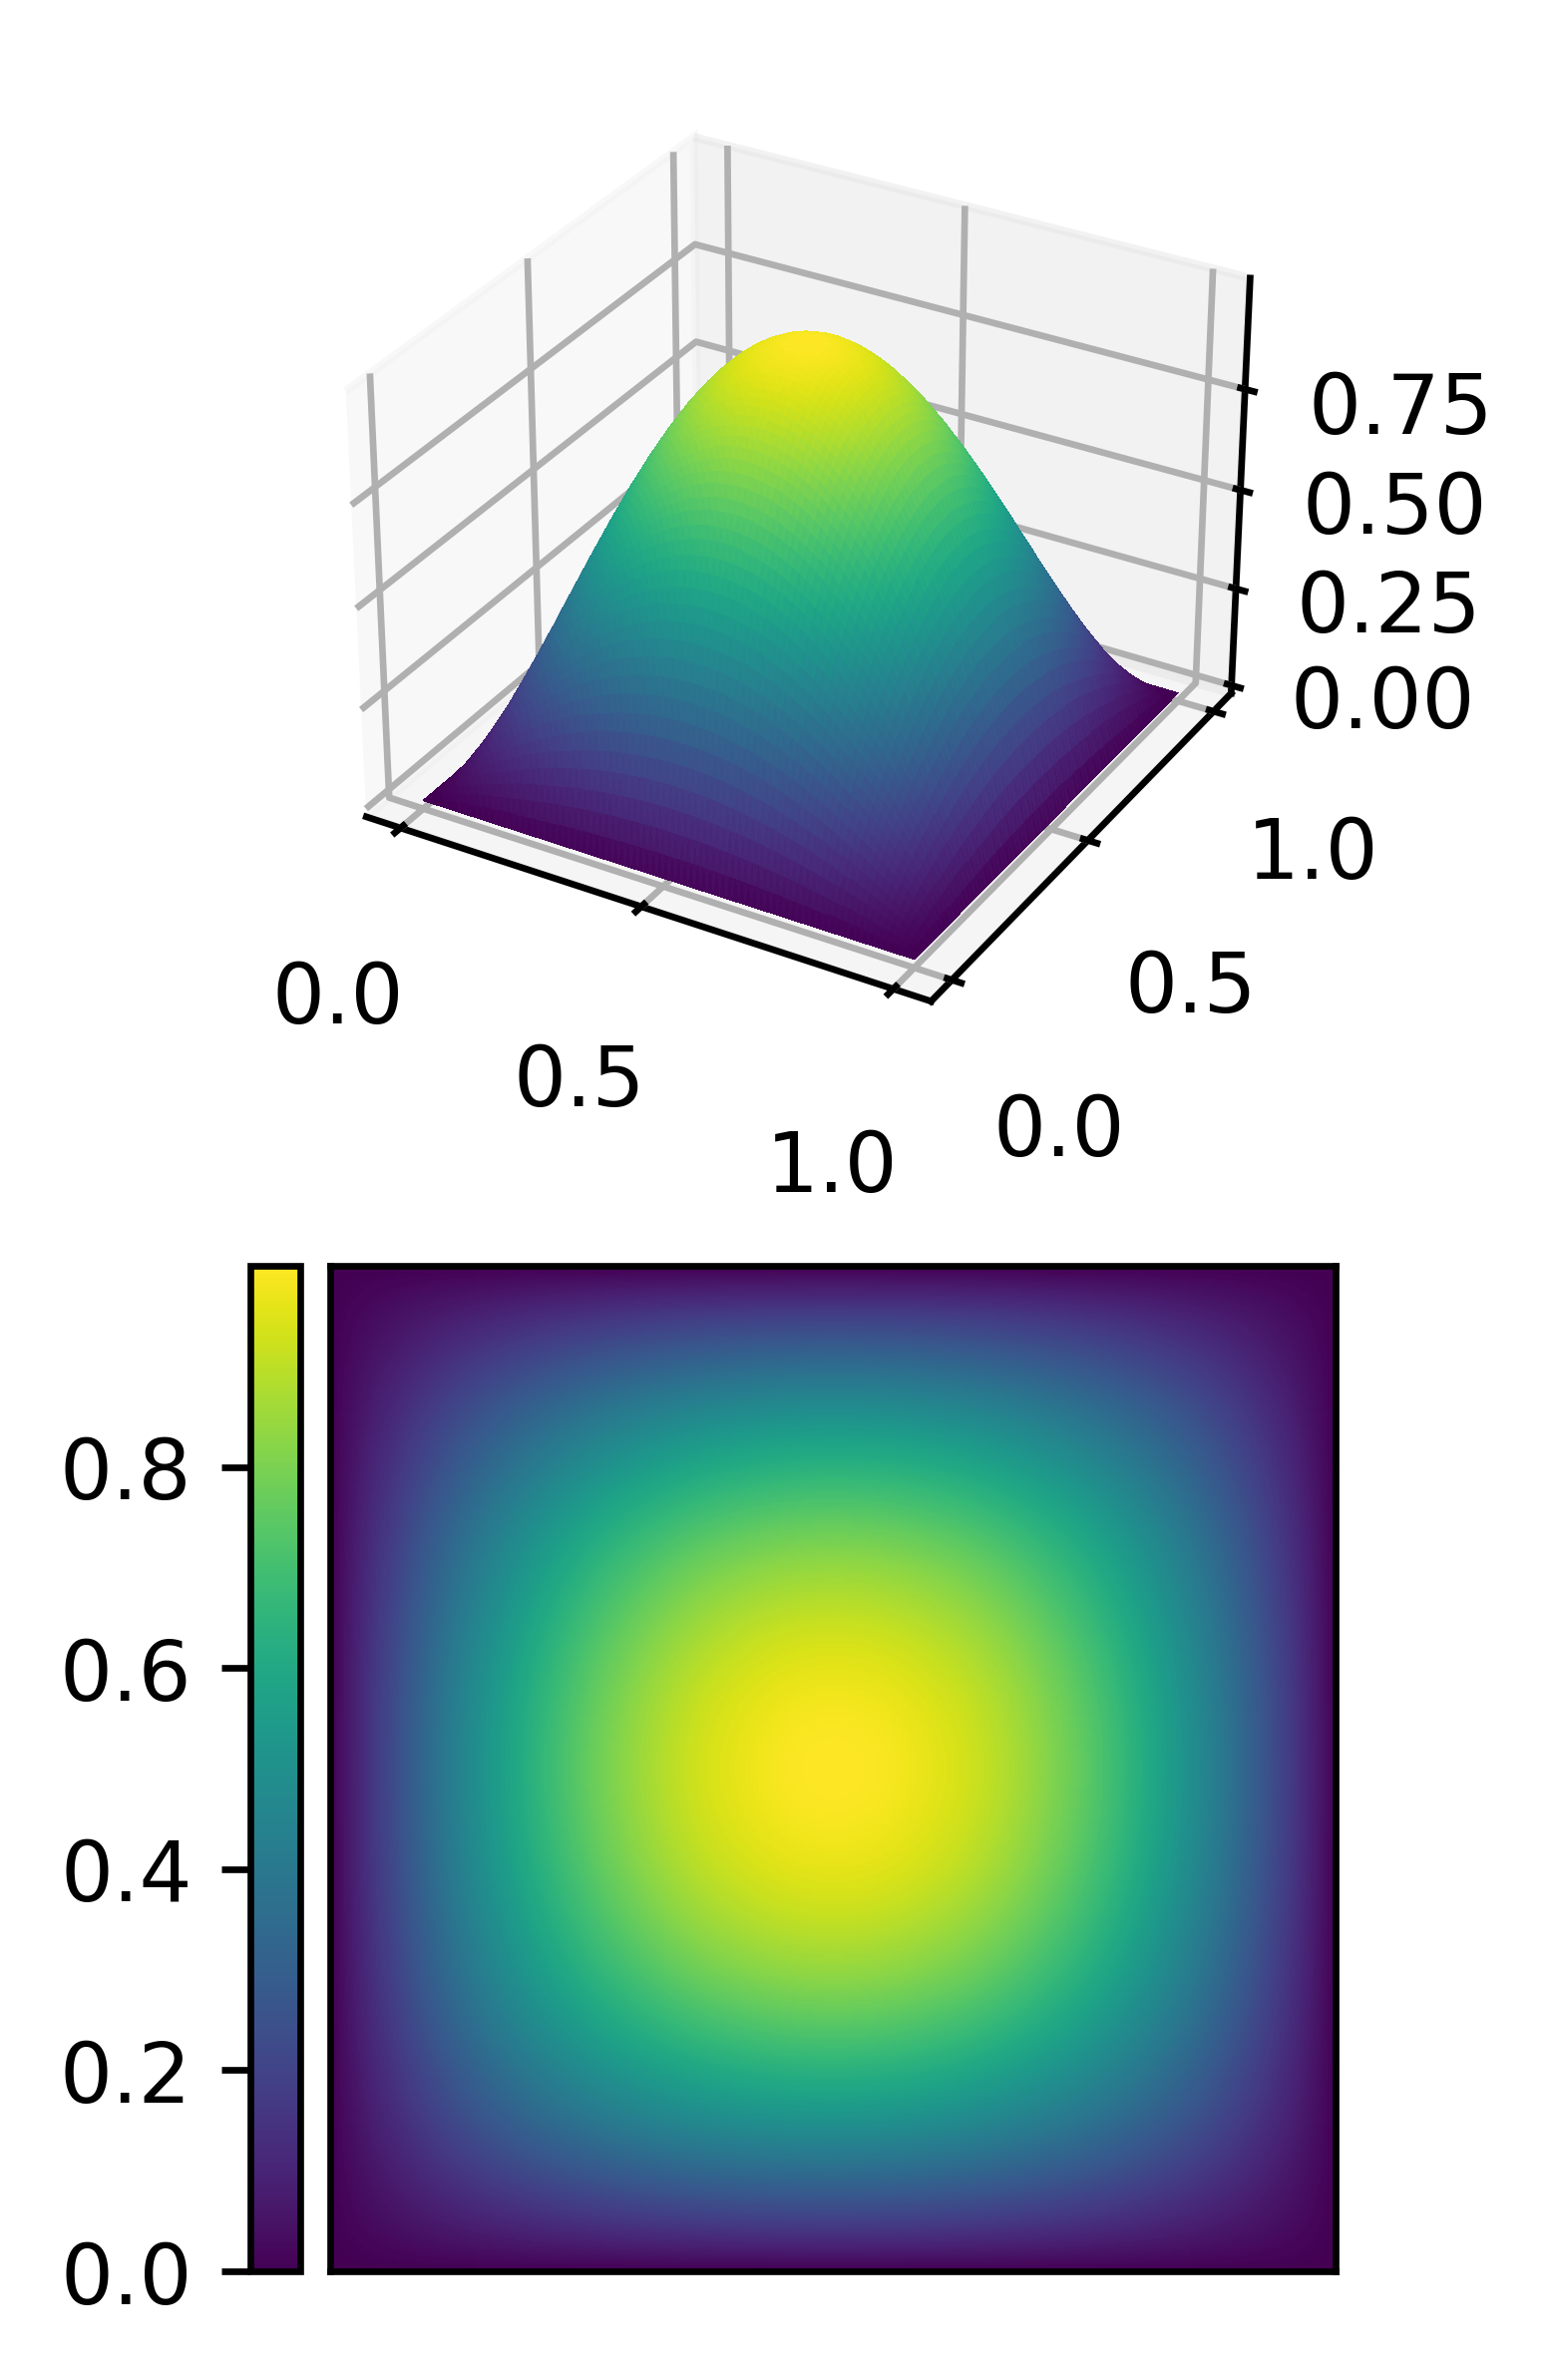
\includegraphics[width=.6\linewidth]{contour_1}
    \caption{$a = 1$}
  \end{subfigure}%
  \begin{subfigure}{.5\textwidth}
    \centering
    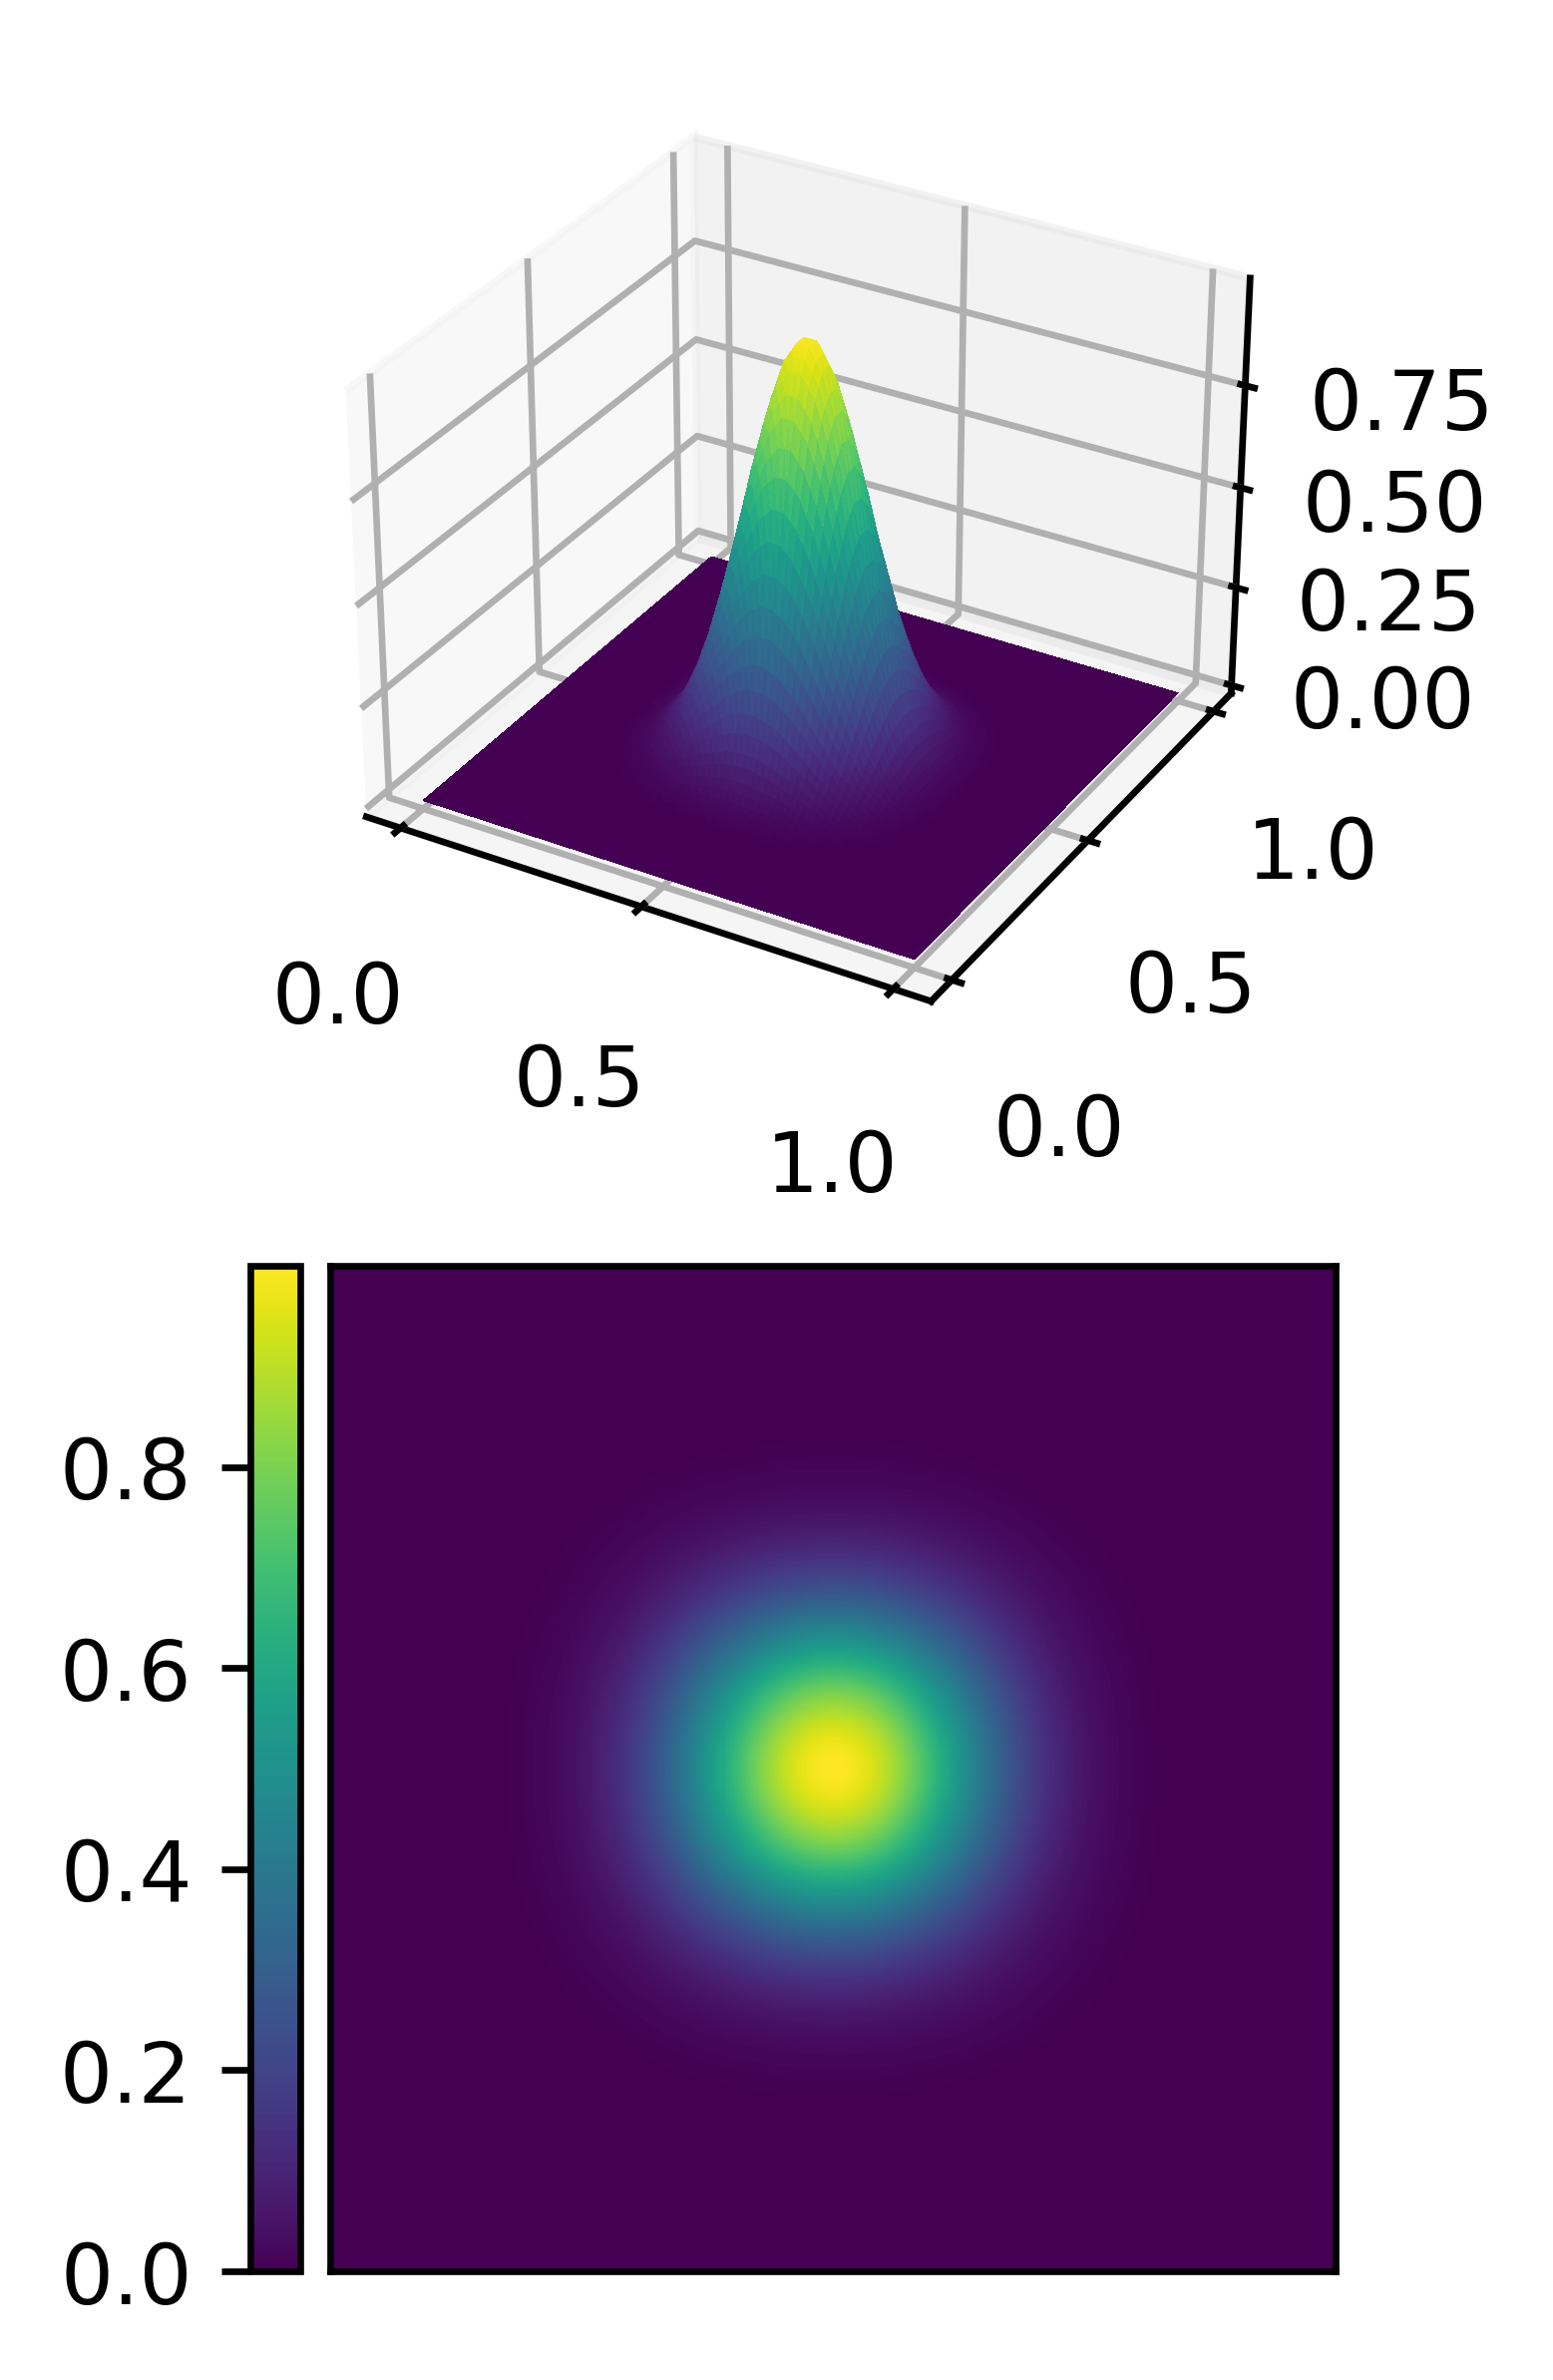
\includegraphics[width=.6\linewidth]{contour_10}
    \caption{$a = 10$}
  \end{subfigure}
  \caption{Solution $u$ with varying parameter $a$}
  \label{fig:smooth_dirichlet_solution}
\end{figure}

\begin{figure}
  \centering
  \begin{subfigure}{.2\textwidth}
    \centering
    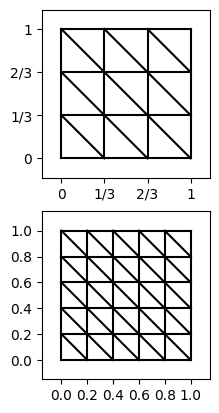
\includegraphics[width=1\linewidth]{structured_grids}
    \caption{Grids for $n=4$ and $n=6$}
  \end{subfigure}%
  \begin{subfigure}{.8\textwidth}
    \centering
    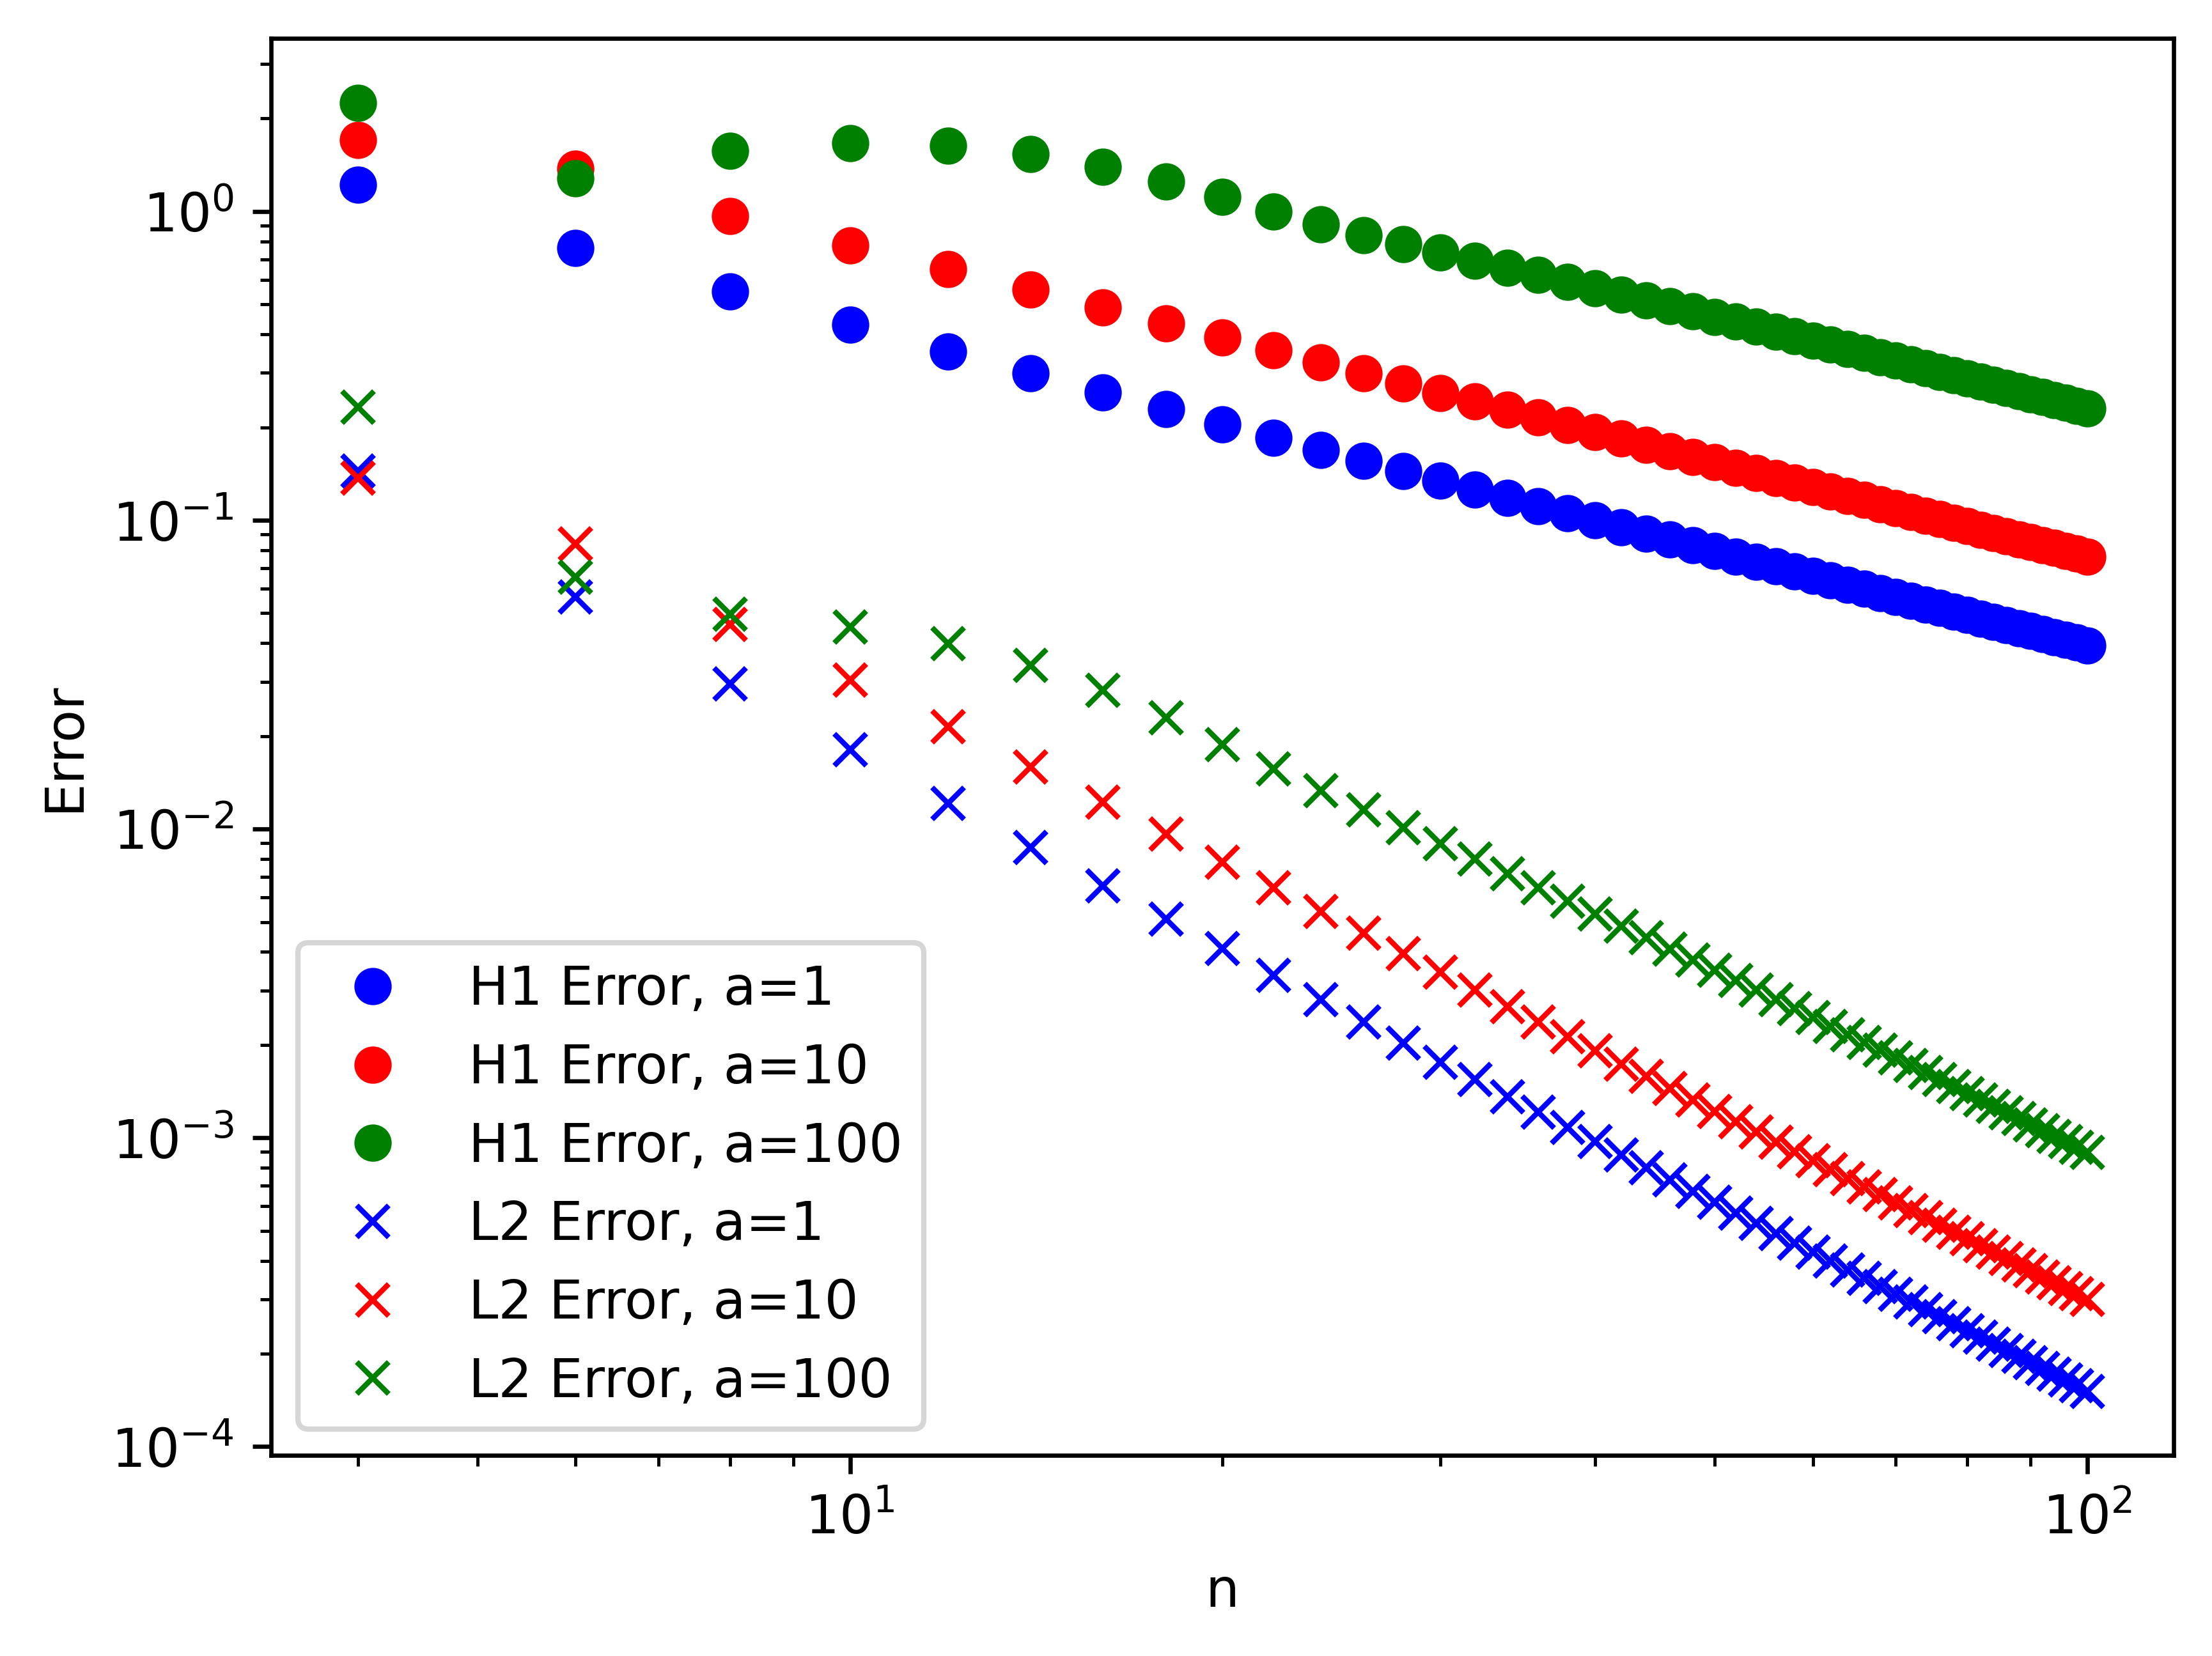
\includegraphics[width=.9\linewidth]{errors_smooth_regular}
    \caption{Error in $H^1$ Semi-Norm with Increasing $H^2$ Norm of $u$}
  \end{subfigure}
  \label{fig:smooth_dirichlet_h1_err}
  \caption{Smooth Solution with Dirichlet Boundary Conditions on a Structured Grid}
\end{figure}

\begin{figure}
  \centering
  \begin{subfigure}{.2\textwidth}
    \centering
    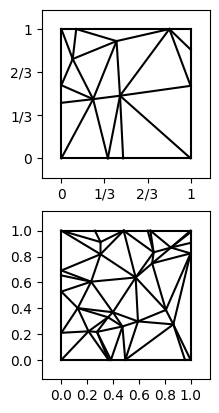
\includegraphics[width=1\linewidth]{unstructured_grids}
    \caption{Grids for $n=4$ and $n=6$}
  \end{subfigure}%
  \begin{subfigure}{.8\textwidth}
    \centering
    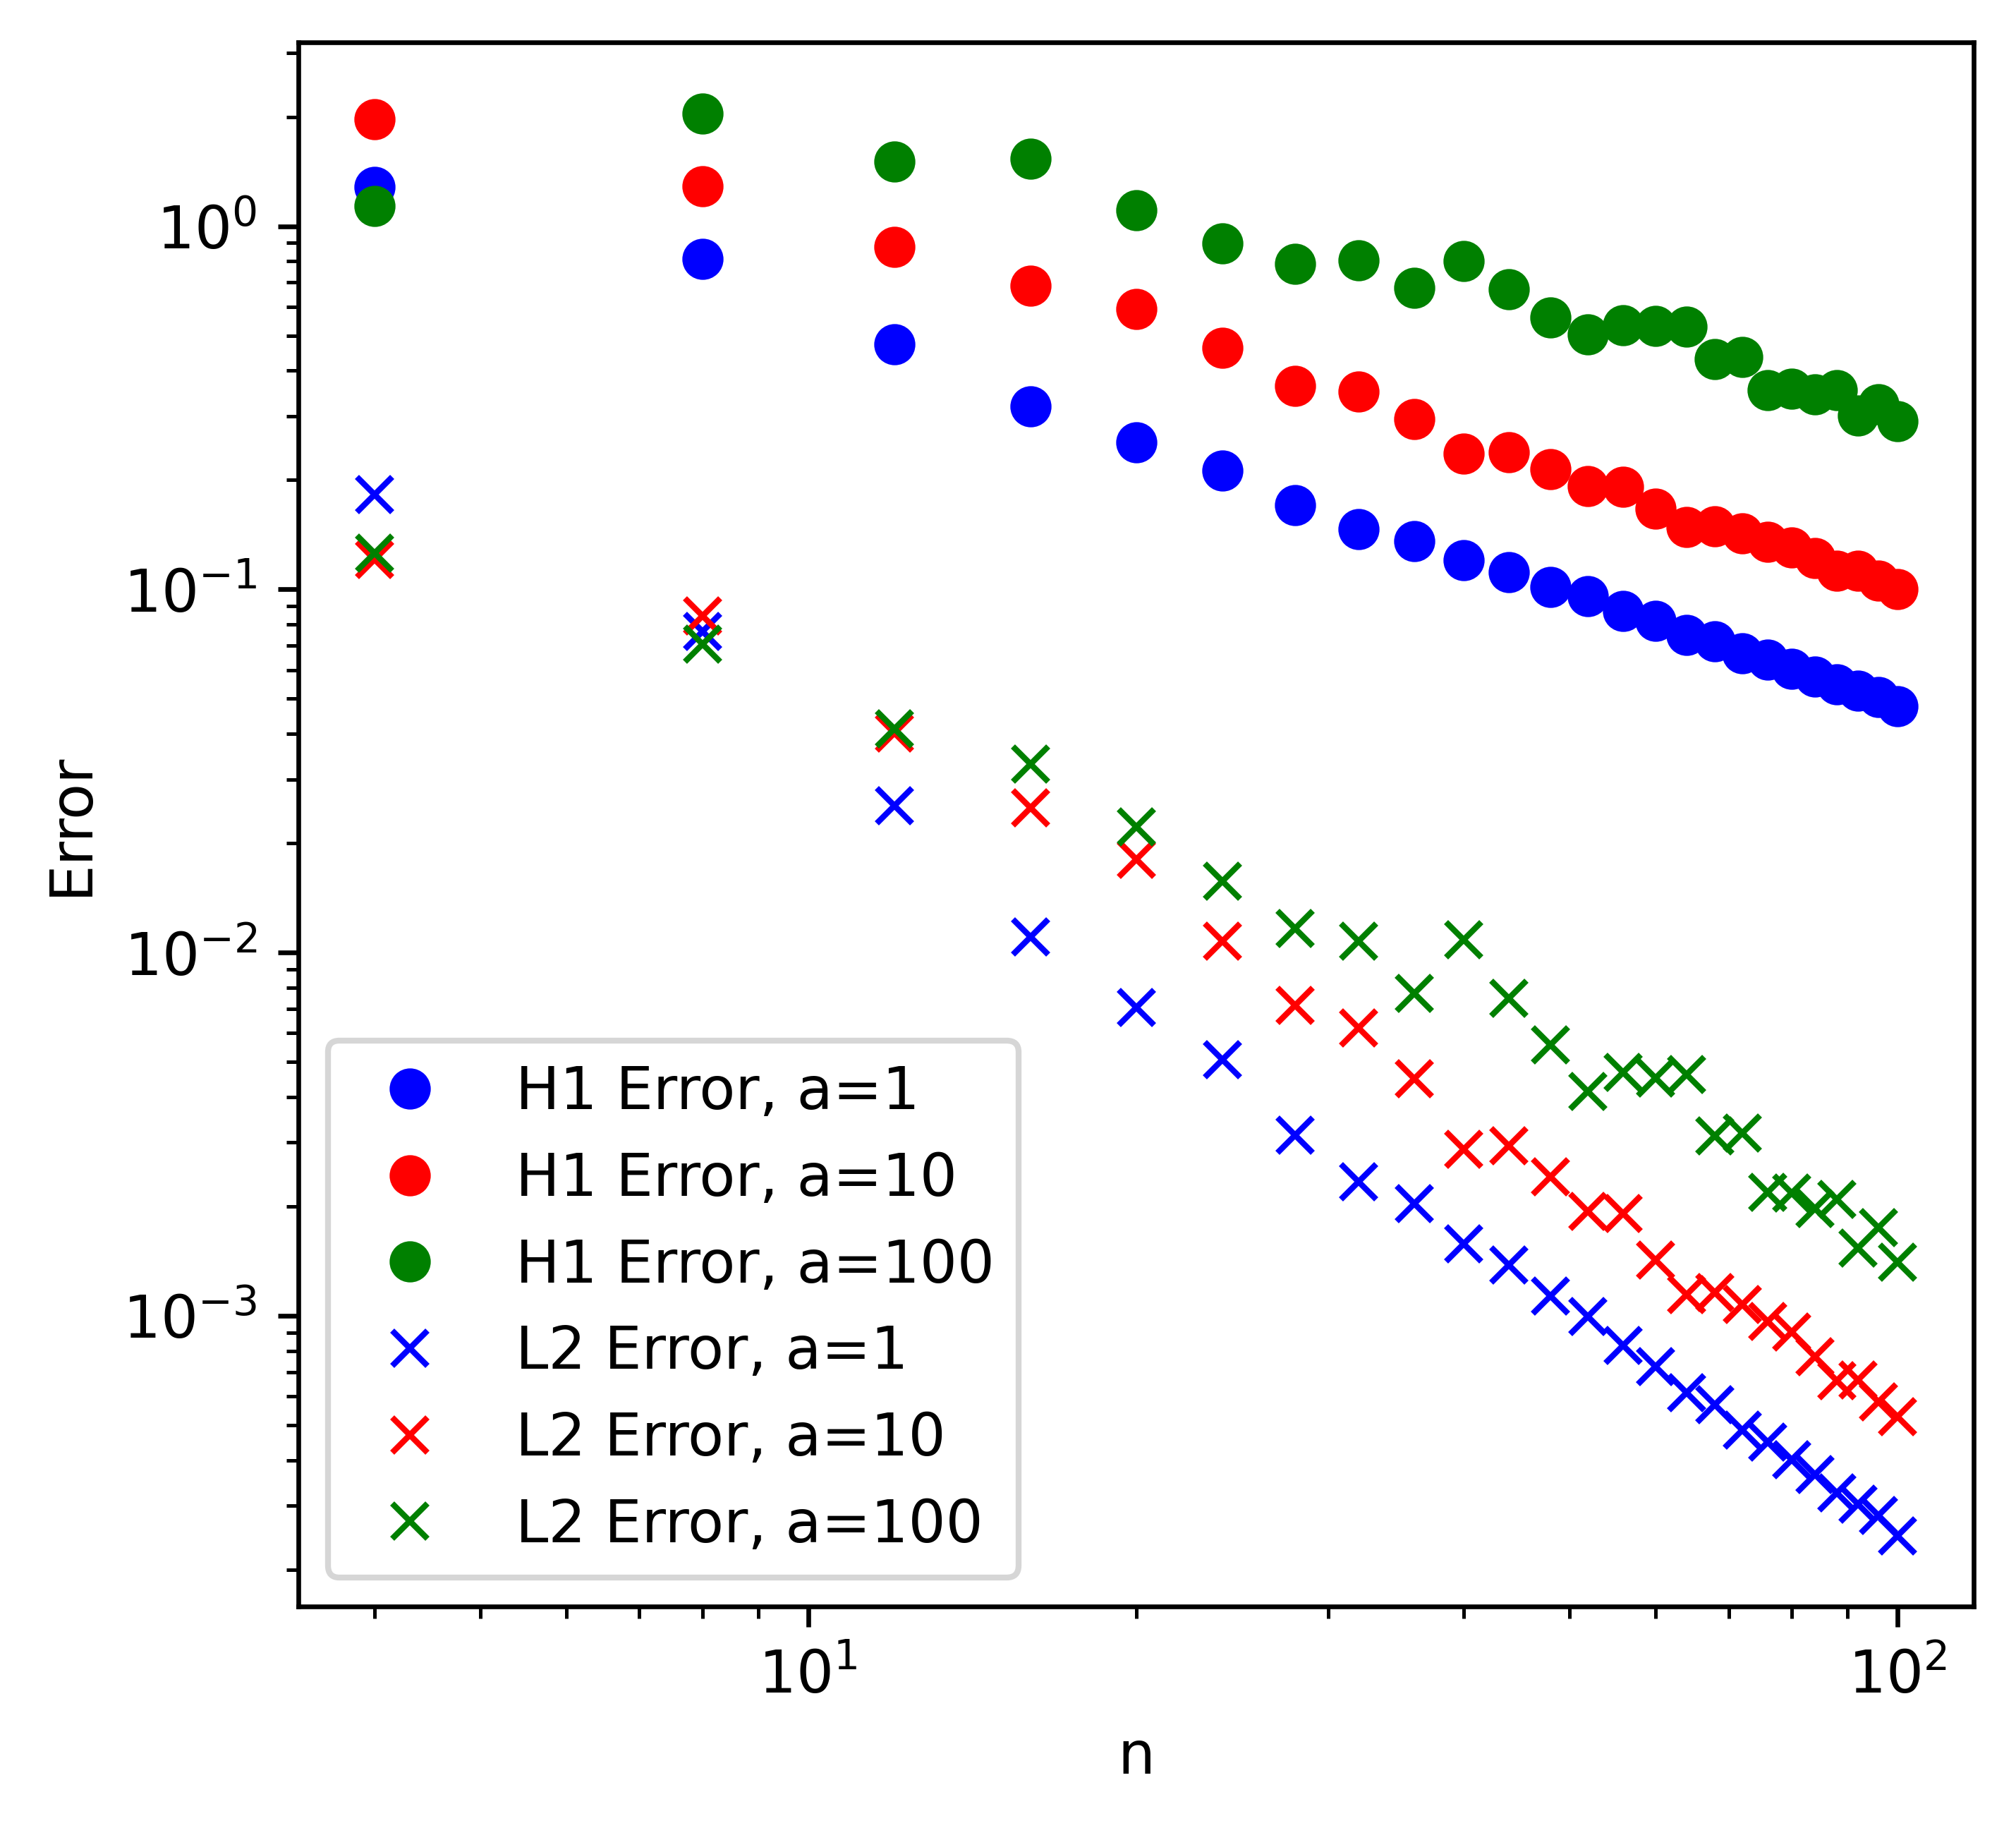
\includegraphics[width=.9\linewidth]{errors_smooth_unstructured}
    \caption{Error in $H^1$ Semi-Norm with Increasing $H^2$ Norm of $u$}
  \end{subfigure}
  \label{fig:smooth_dirichlet_h1_err}
  \caption{Smooth Solution with Dirichlet Boundary Conditions on an Unstructured Grid}
\end{figure}


\subsection*{Neumann Boundary Conditions}
Considering the following problem with mixed Dirichlet and Neumann boundary conditions.
\begin{equation}
  \begin{split}
    \Omega &= \left[-1,1\right]^2\\
    -\Delta u &= \begin{cases}
      \frac{\pi^2}{4} \operatorname{cos}\left(\frac{\pi}{2} \cdot y\right) \quad &x \le 0\\
      \frac{\pi^2}{4} \operatorname{cos}\left(\frac{\pi}{2} \cdot y\right) - a\left(a-1\right)x^{a-2} \quad &x > 0
    \end{cases}\\
    u(x,y) &= 0 \quad \text{on } [-1,0] \times -1\\
    u(x,y) &= x^a \quad \text{on } (0,1] \times -1\\
    u(x,y) &= 0 \quad \text{on } [-1,0] \times 1\\
    u(x,y) &= x^a \quad \text{on } (0,1] \times 1\\
    \frac{\partial u}{\partial {\bf n}} &= 0 \quad \text{on } -1 \times (-1,1)\\
    \frac{\partial u}{\partial {\bf n}} &= a \quad \text{on } 1 \times (-1,1)
  \end{split}
\end{equation}
With known solution:
\begin{equation*}
  u(x,y) = \begin{cases}
    \operatorname{cos}\left(\frac{\pi}{2} \cdot y\right) \quad &x \le 0\\
    \operatorname{cos}\left(\frac{\pi}{2} \cdot y\right) + x^a \quad &x > 0
  \end{cases}
\end{equation*}

Where $u \in H^{a+0.5 - \epsilon}(\Omega) \quad \forall \epsilon > 0$. With increasing $a$,
the function $\Delta u$ will develop a singularity along the $x = 0$ line. For the previous convergence
results to be meaningful we need $a > 1$, so $u$ is continuous and the interpolation operator
well-defined.\\
The regularity of the Dirichlet boundary is also controlled by $a$. For a solution to be found,
only square integrability on the boundary is needed. Therefore, the solution is not affected by this.

\begin{figure}
  \centering
  \begin{subfigure}{.5\textwidth}
    \centering
    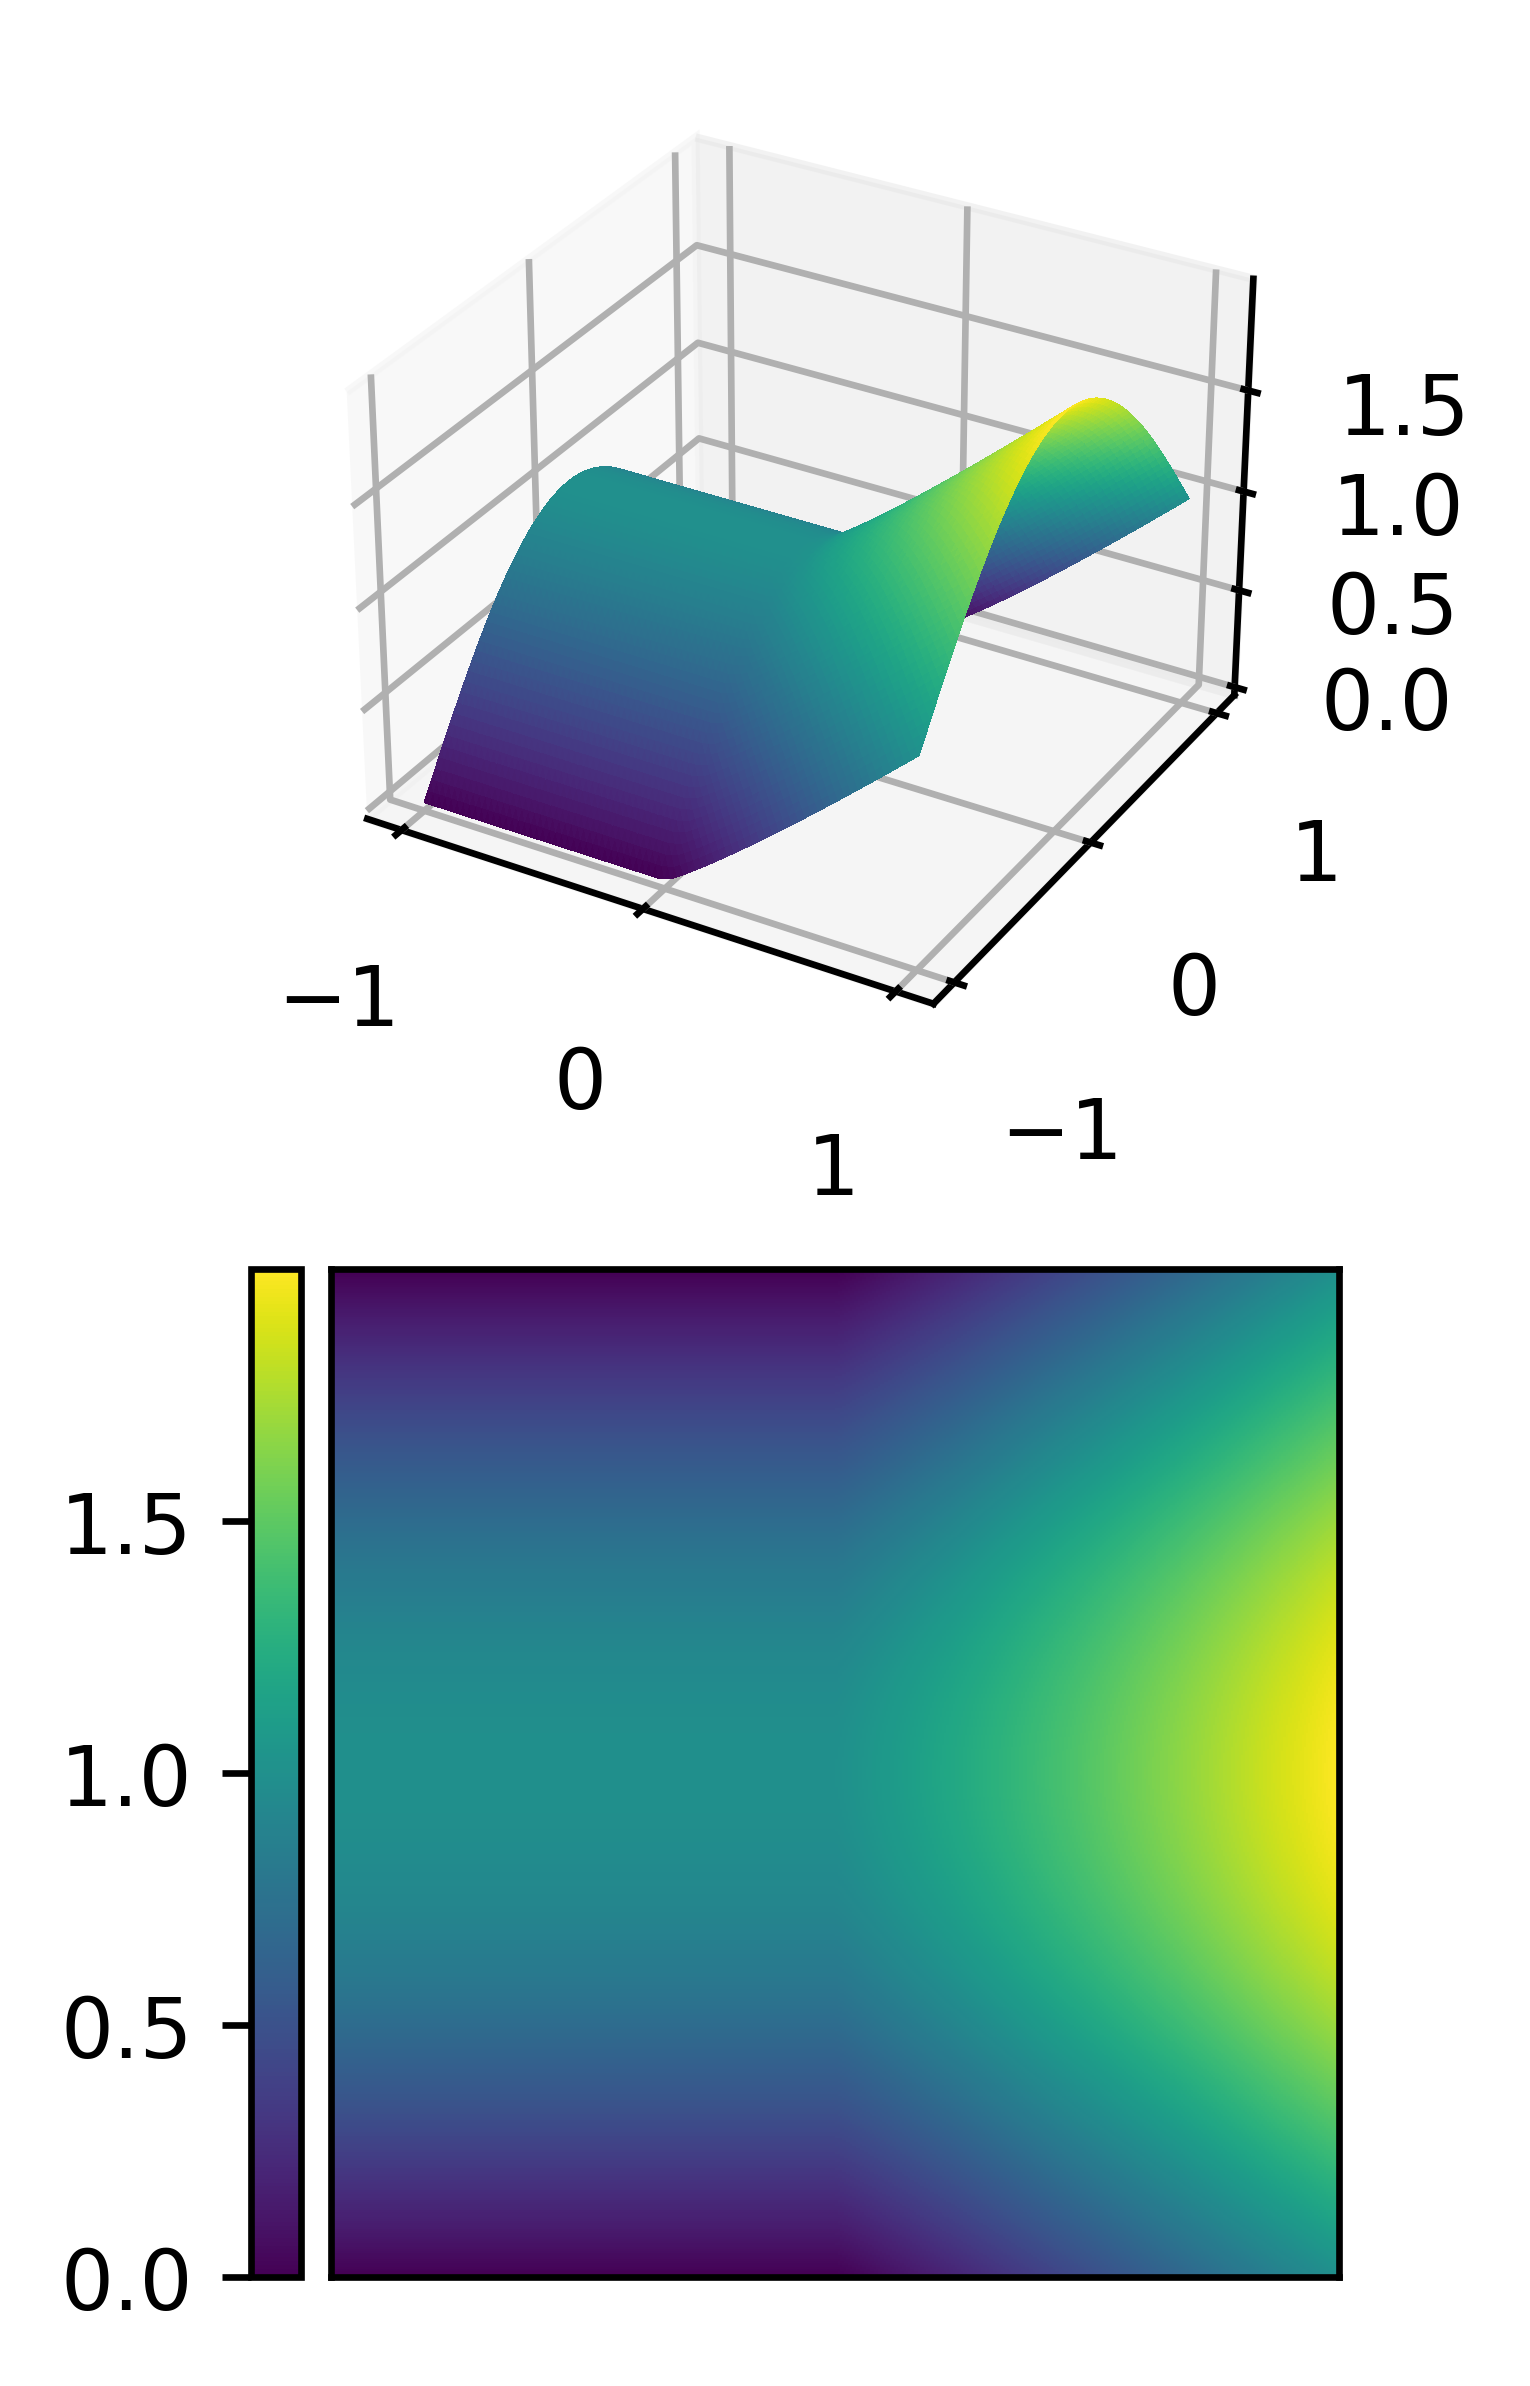
\includegraphics[width=.6\linewidth]{contour_nonsmooth_1}
    \caption{$a = 1.1$}
  \end{subfigure}%
  \begin{subfigure}{.5\textwidth}
    \centering
    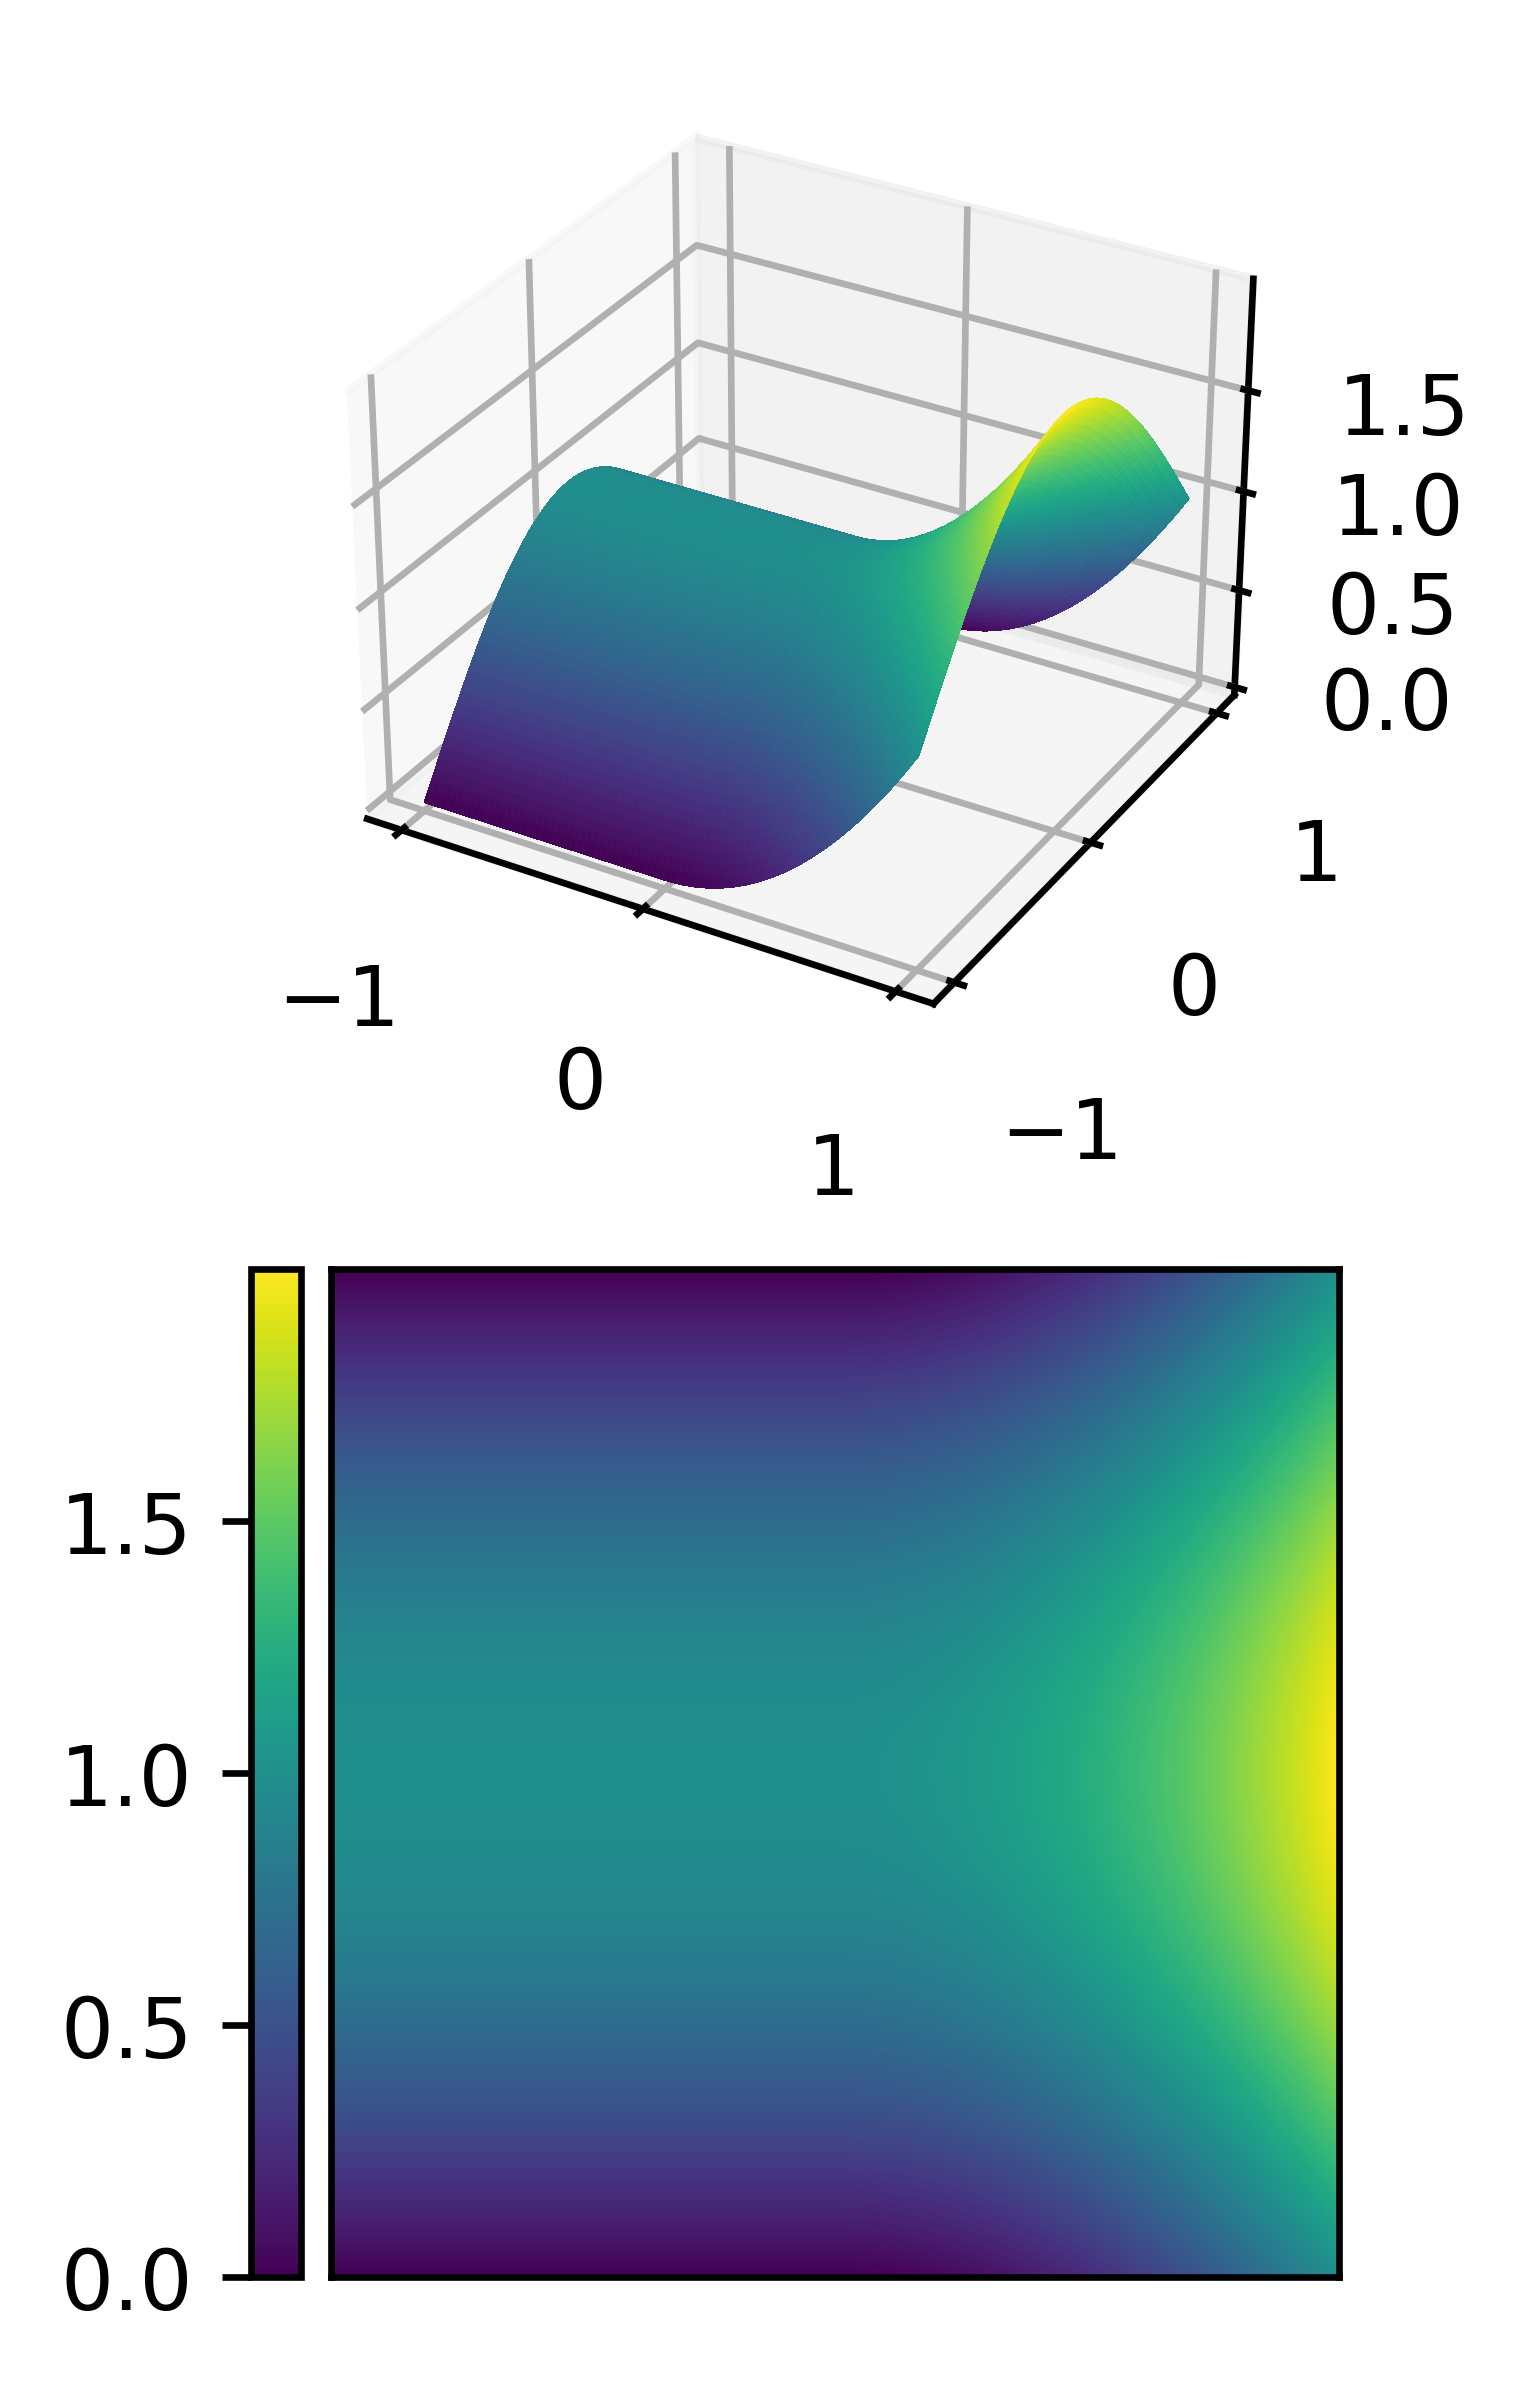
\includegraphics[width=.6\linewidth]{contour_nonsmooth_2}
    \caption{$a = 2$}
  \end{subfigure}
  \caption{Solution $u$ with varying parameter $a$}
  \label{fig:non_smooth_mixed_solution}
\end{figure}

For $1 < a \le 1.5$ we have $u \notin H^2(\Omega)$ and therefore no convergence estimate at hand.
For $1.5 < a$ linear convergence in the $H^1$ semi-norm is expected.
For convergence in the $L^2$ norm the theorem guaranteeing a convergence estimates
in its precise form states:
\begin{equation}
  \begin{split}
    &\exists n \in \mathbb{N}: \, \lVert u - u_h \rVert_{L^2} \in \mathcal{O}\left(h\right), \quad \forall h < \frac{1}{n}, u \in H^1(\Omega) \\
    &\exists n \in \mathbb{N}: \, \lVert u - u_h \rVert_{L^2} \in \mathcal{O}\left(h^2\right), \quad \forall h < \frac{1}{n}, u \in H^2(\Omega) \\
  \end{split}
\end{equation}
This threshold is likely to increase with less regularity of the solution. So a more natural
expectation is for the convergence rate to increase with increasing $a$.
Both of this is observed in the numerical experiment. As visualized in \ref{fig:err_nonsmooth_h1},
the convergence rate for the $H^1$ semi-norm is exactly linear for $1.5 < a$.
For $a = 1.3$ the method is still guaranteed to converge, although no convergence estimate can be established.
From the numerical experiment it appears to converge at a rate $\mathcal{O}\left(h^{0.6}\right)$.

In \ref{fig:err_nonsmooth_l2} it can be seen how the convergence rate depends on the regularity of the solution.
Although, for $1.5 < a$ quadratic convergence is eventually guaranteed, $n = 100$ is definitely too small.
Truly quadratic convergence can only be observed for $2.2 < a$
\begin{figure}
  \centering
  \begin{subfigure}{1\textwidth}
    \centering
    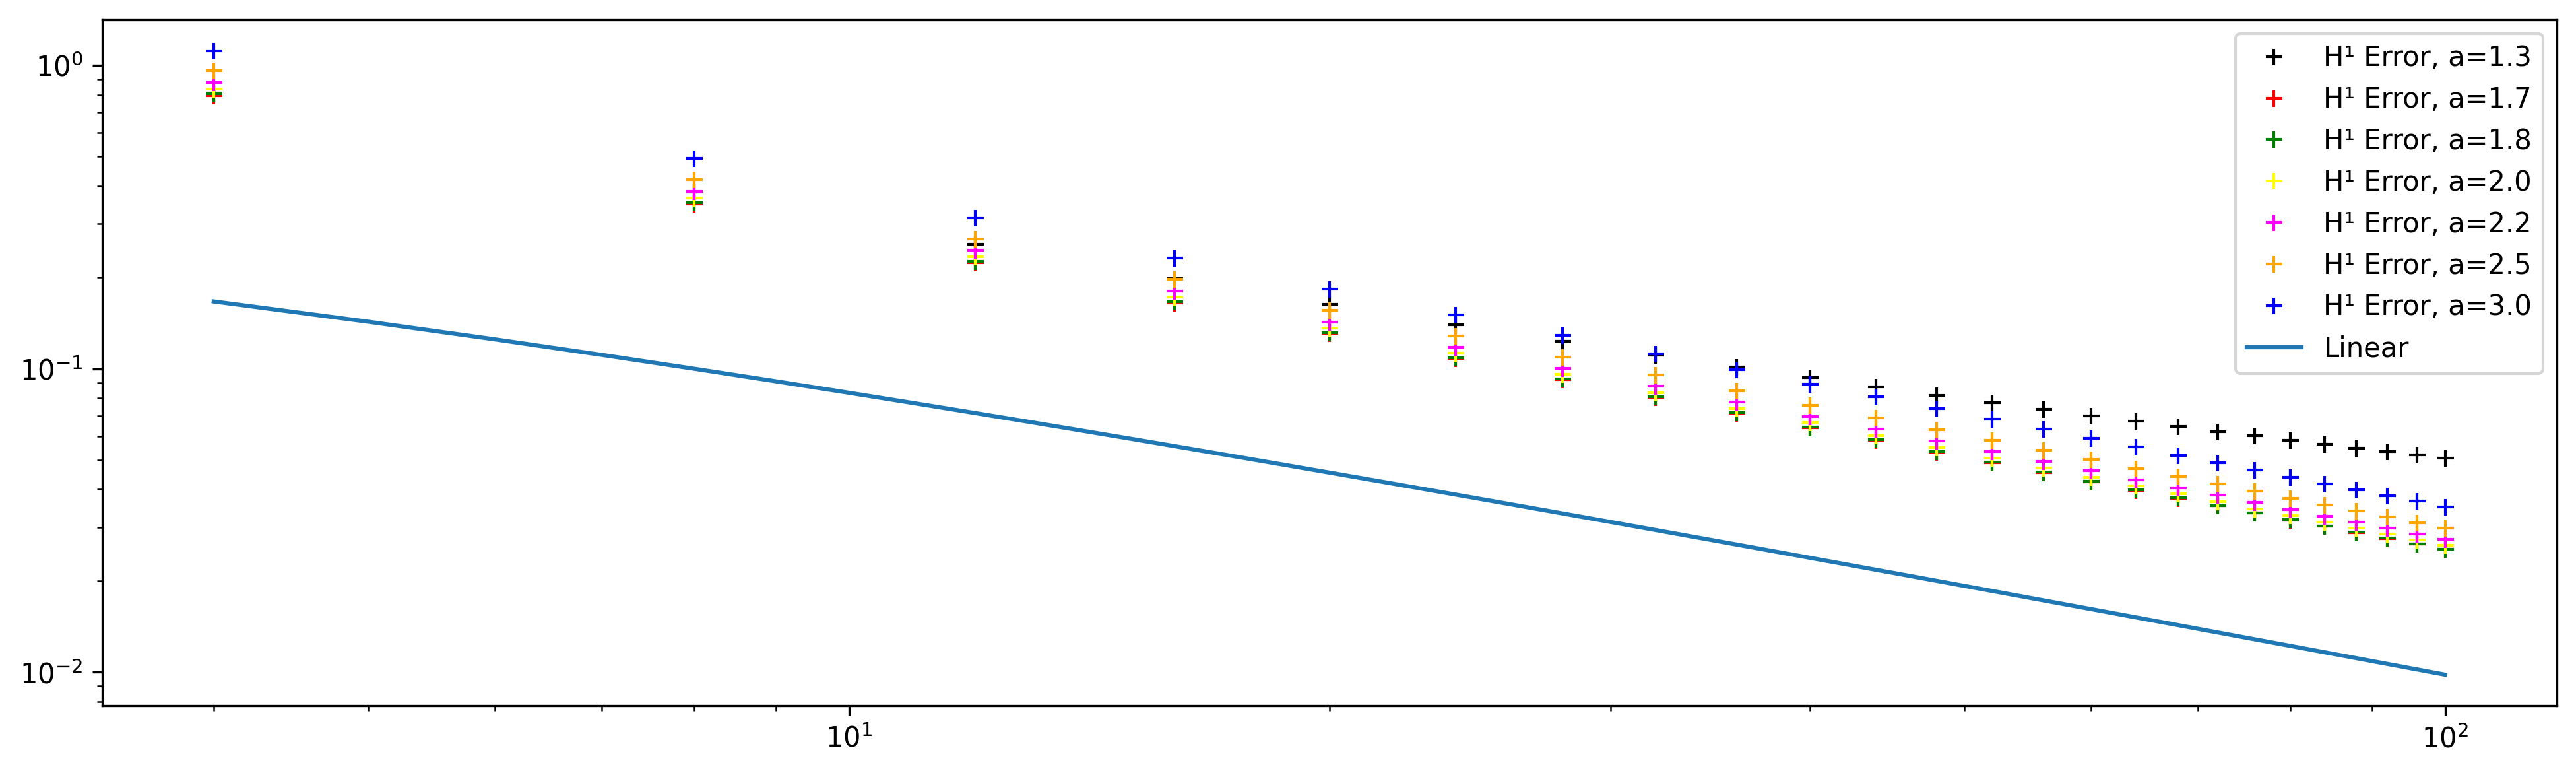
\includegraphics[width=.8\linewidth]{errors_nonsmooth_h1}
    \caption{Convergence in the $H^1$ Semi-Norm}
    \label{fig:err_nonsmooth_h1}
  \end{subfigure}

  \begin{subfigure}{1\textwidth}
    \centering
    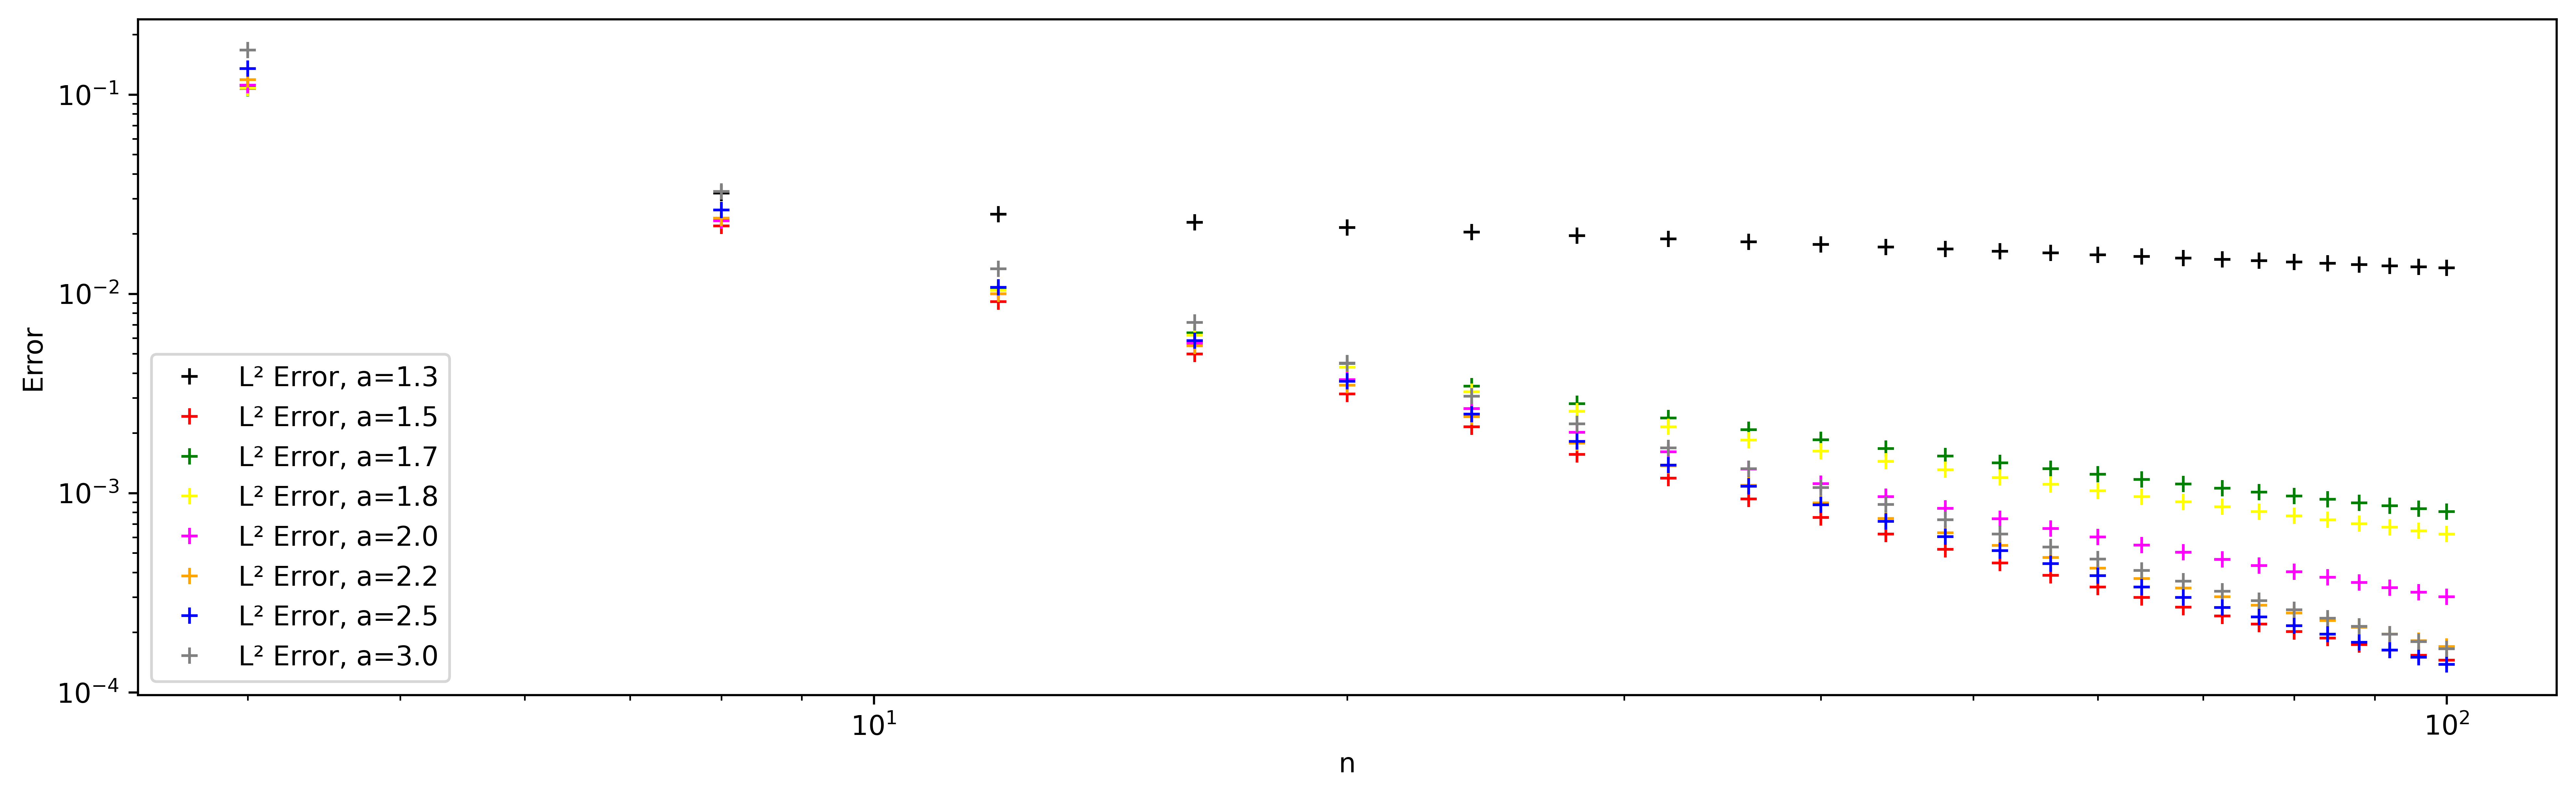
\includegraphics[width=.8\linewidth]{errors_nonsmooth_l2}
    \caption{Convergence in the $L^2$ Norm}
    \label{fig:err_nonsmooth_l2}
  \end{subfigure}
  \caption{Convergence With Varying Regularity of the Solution}
\end{figure}


\subsection*{Higher Order Elements}
To increase the accuracy of the solution on a coarser mesh, a polynomial basis
of higher order can be chosen. This can be achieved by considering higher order local
basis functions defined on the reference element. The local basis functions on the reference
element in 1 and 2 dimension are visualized for 1, 2 and 3 order polynomials in \ref{fig:basis_1d}
and \ref{fig:basis_2d}.
The 3 order Polynomial basis functions for 2 spatial dimensions are omitted, due to the
large amount of basis functions.

\begin{figure}
  \centering
  \begin{subfigure}{1.\textwidth}
    \centering
    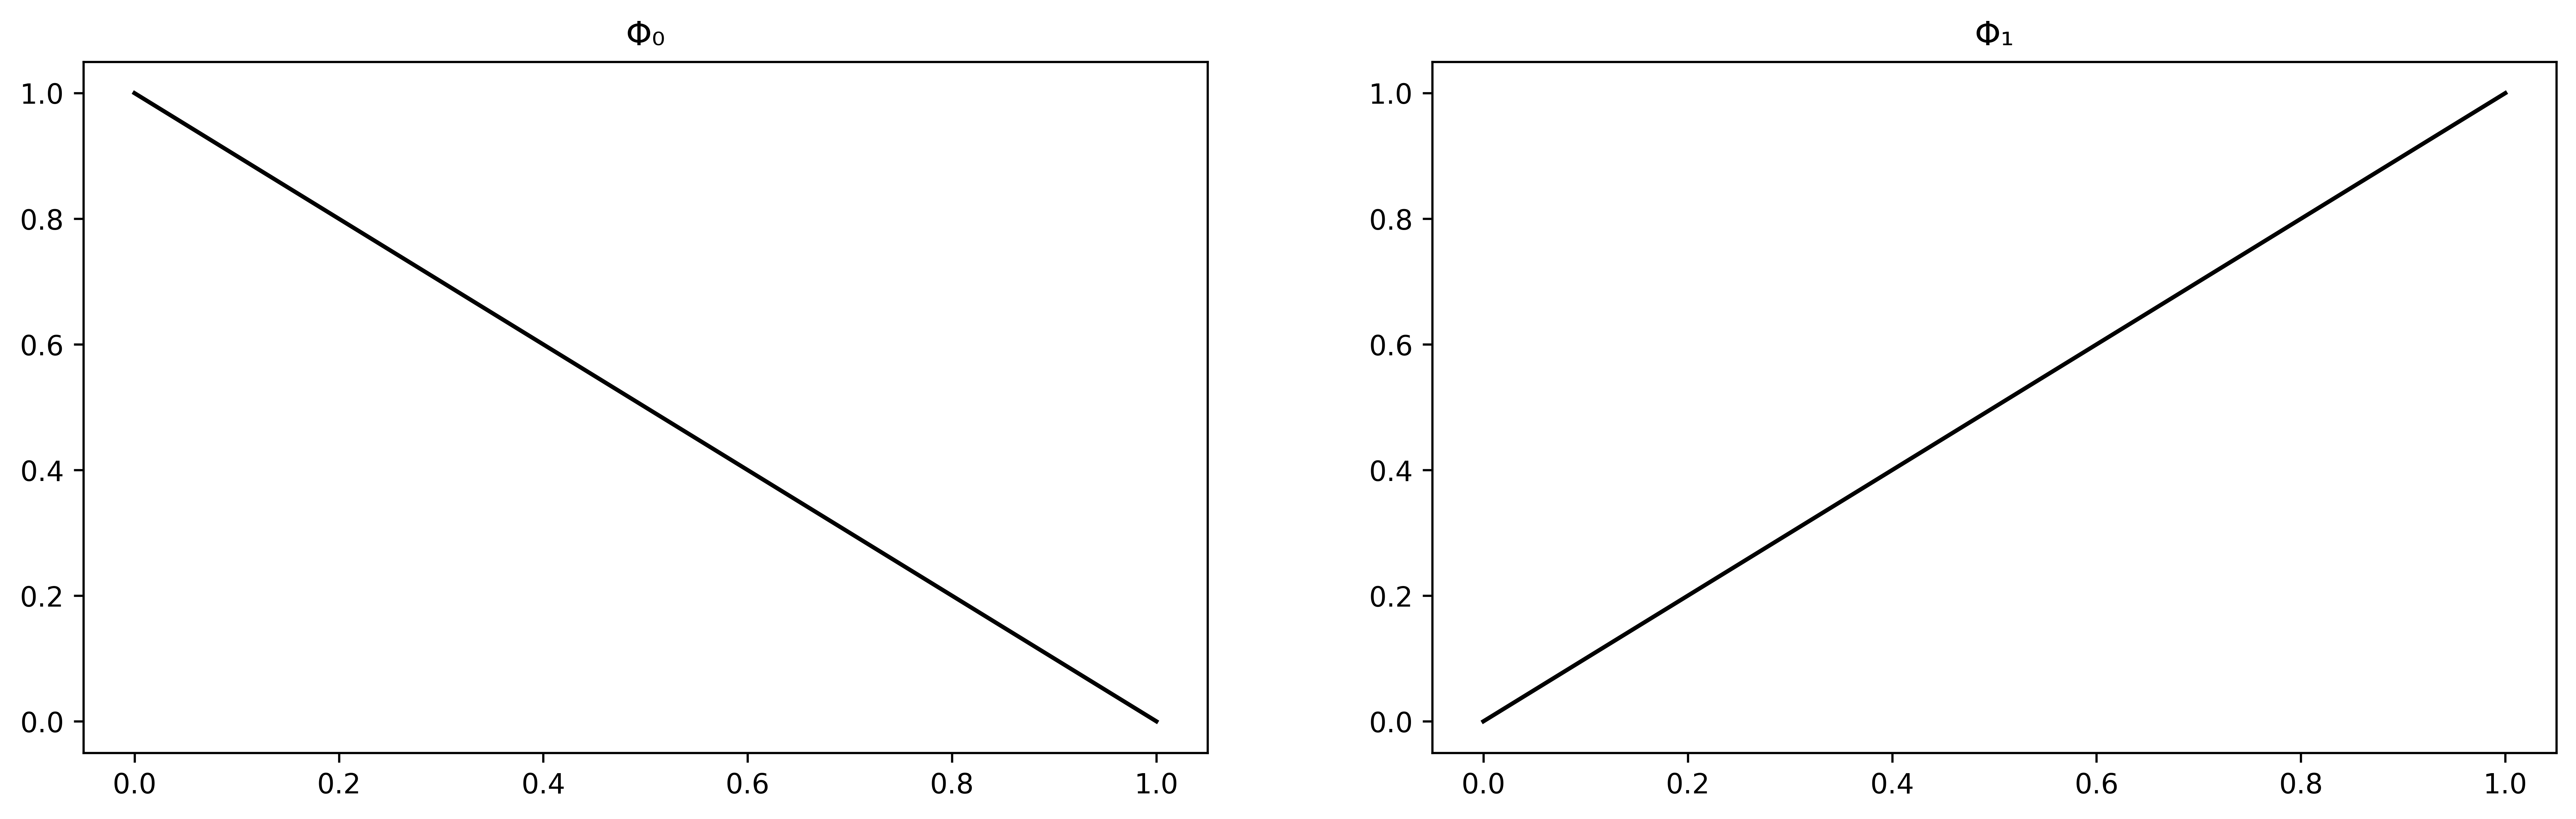
\includegraphics[width=.8\linewidth]{p1_mesh_basis}
    \caption{Polynomial of degree 1 on the unit interval}
  \end{subfigure}
  \begin{subfigure}{1.\textwidth}
    \centering
    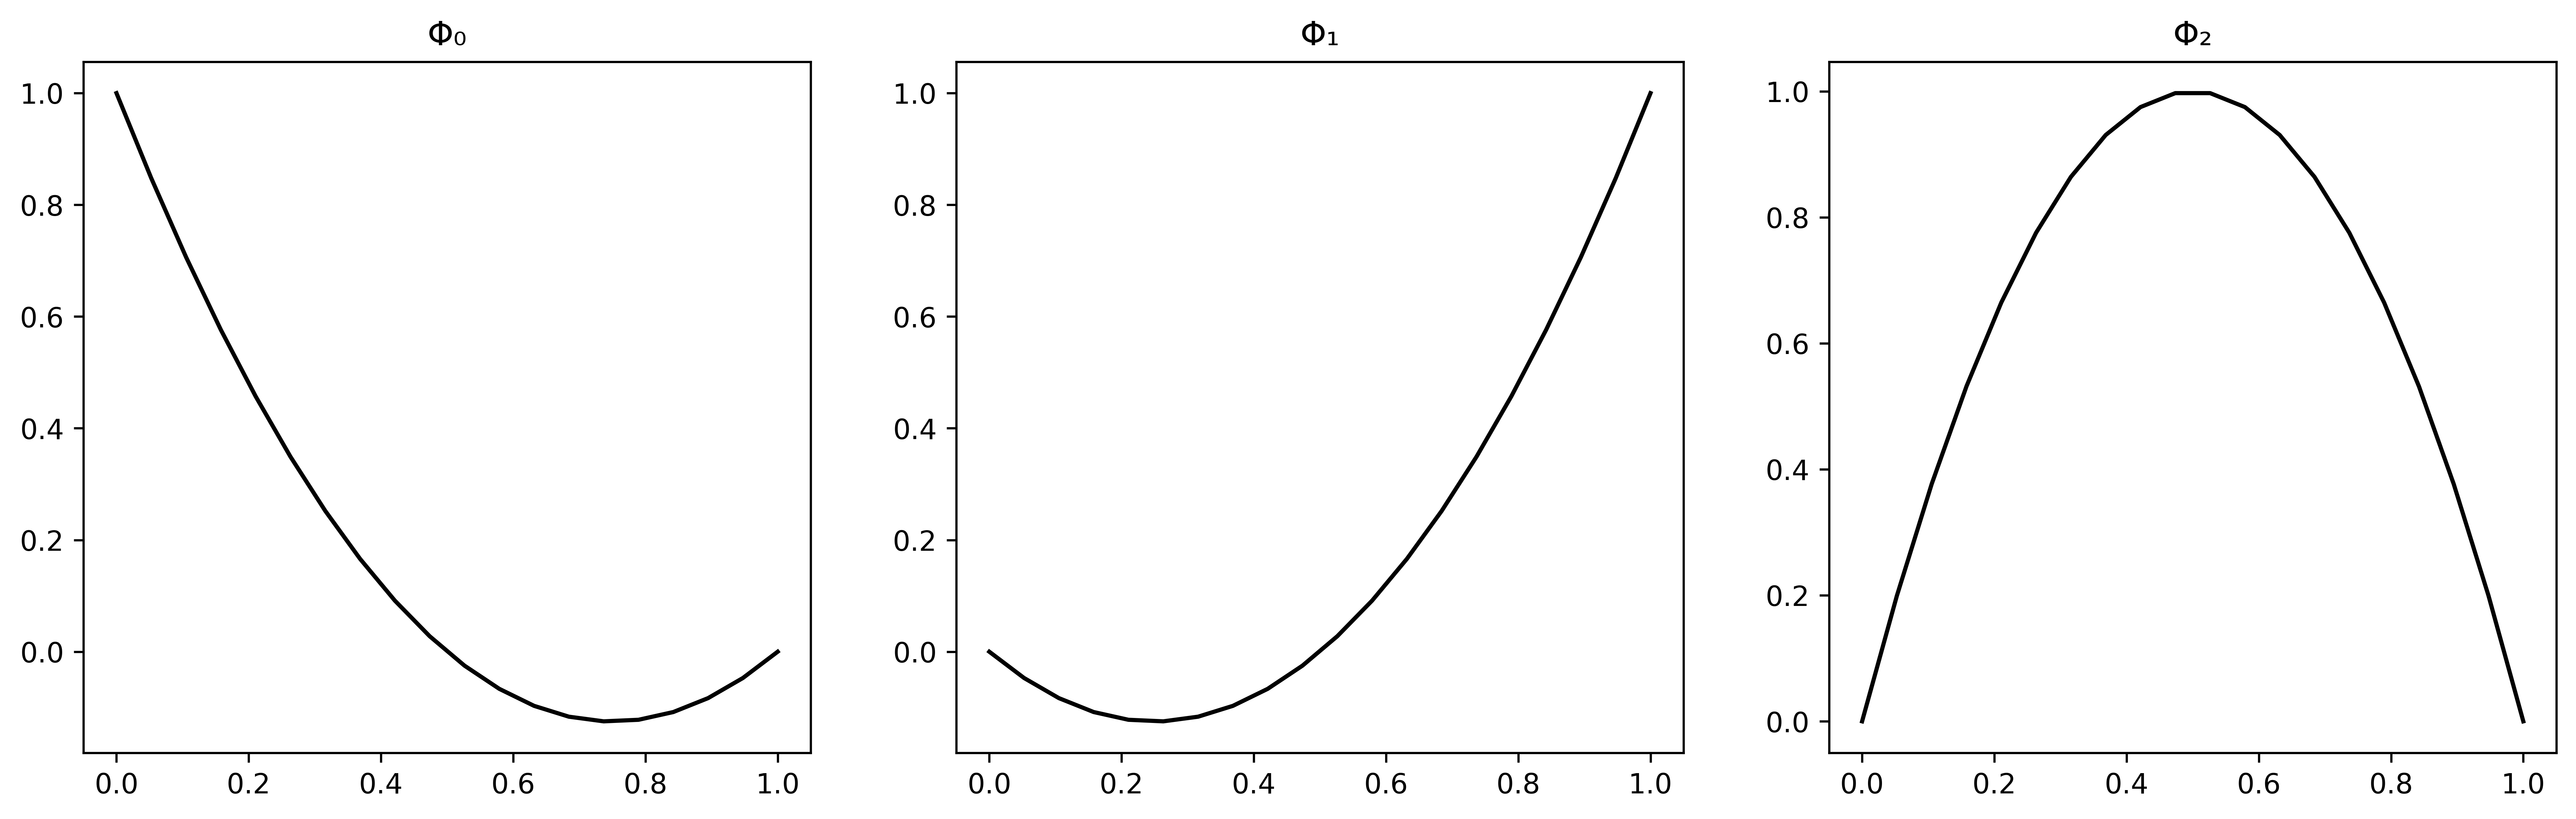
\includegraphics[width=.8\linewidth]{p2_mesh_basis}
    \caption{Polynomial of degree 2 on the unit interval}
  \end{subfigure}
  \begin{subfigure}{1.\textwidth}
    \centering
    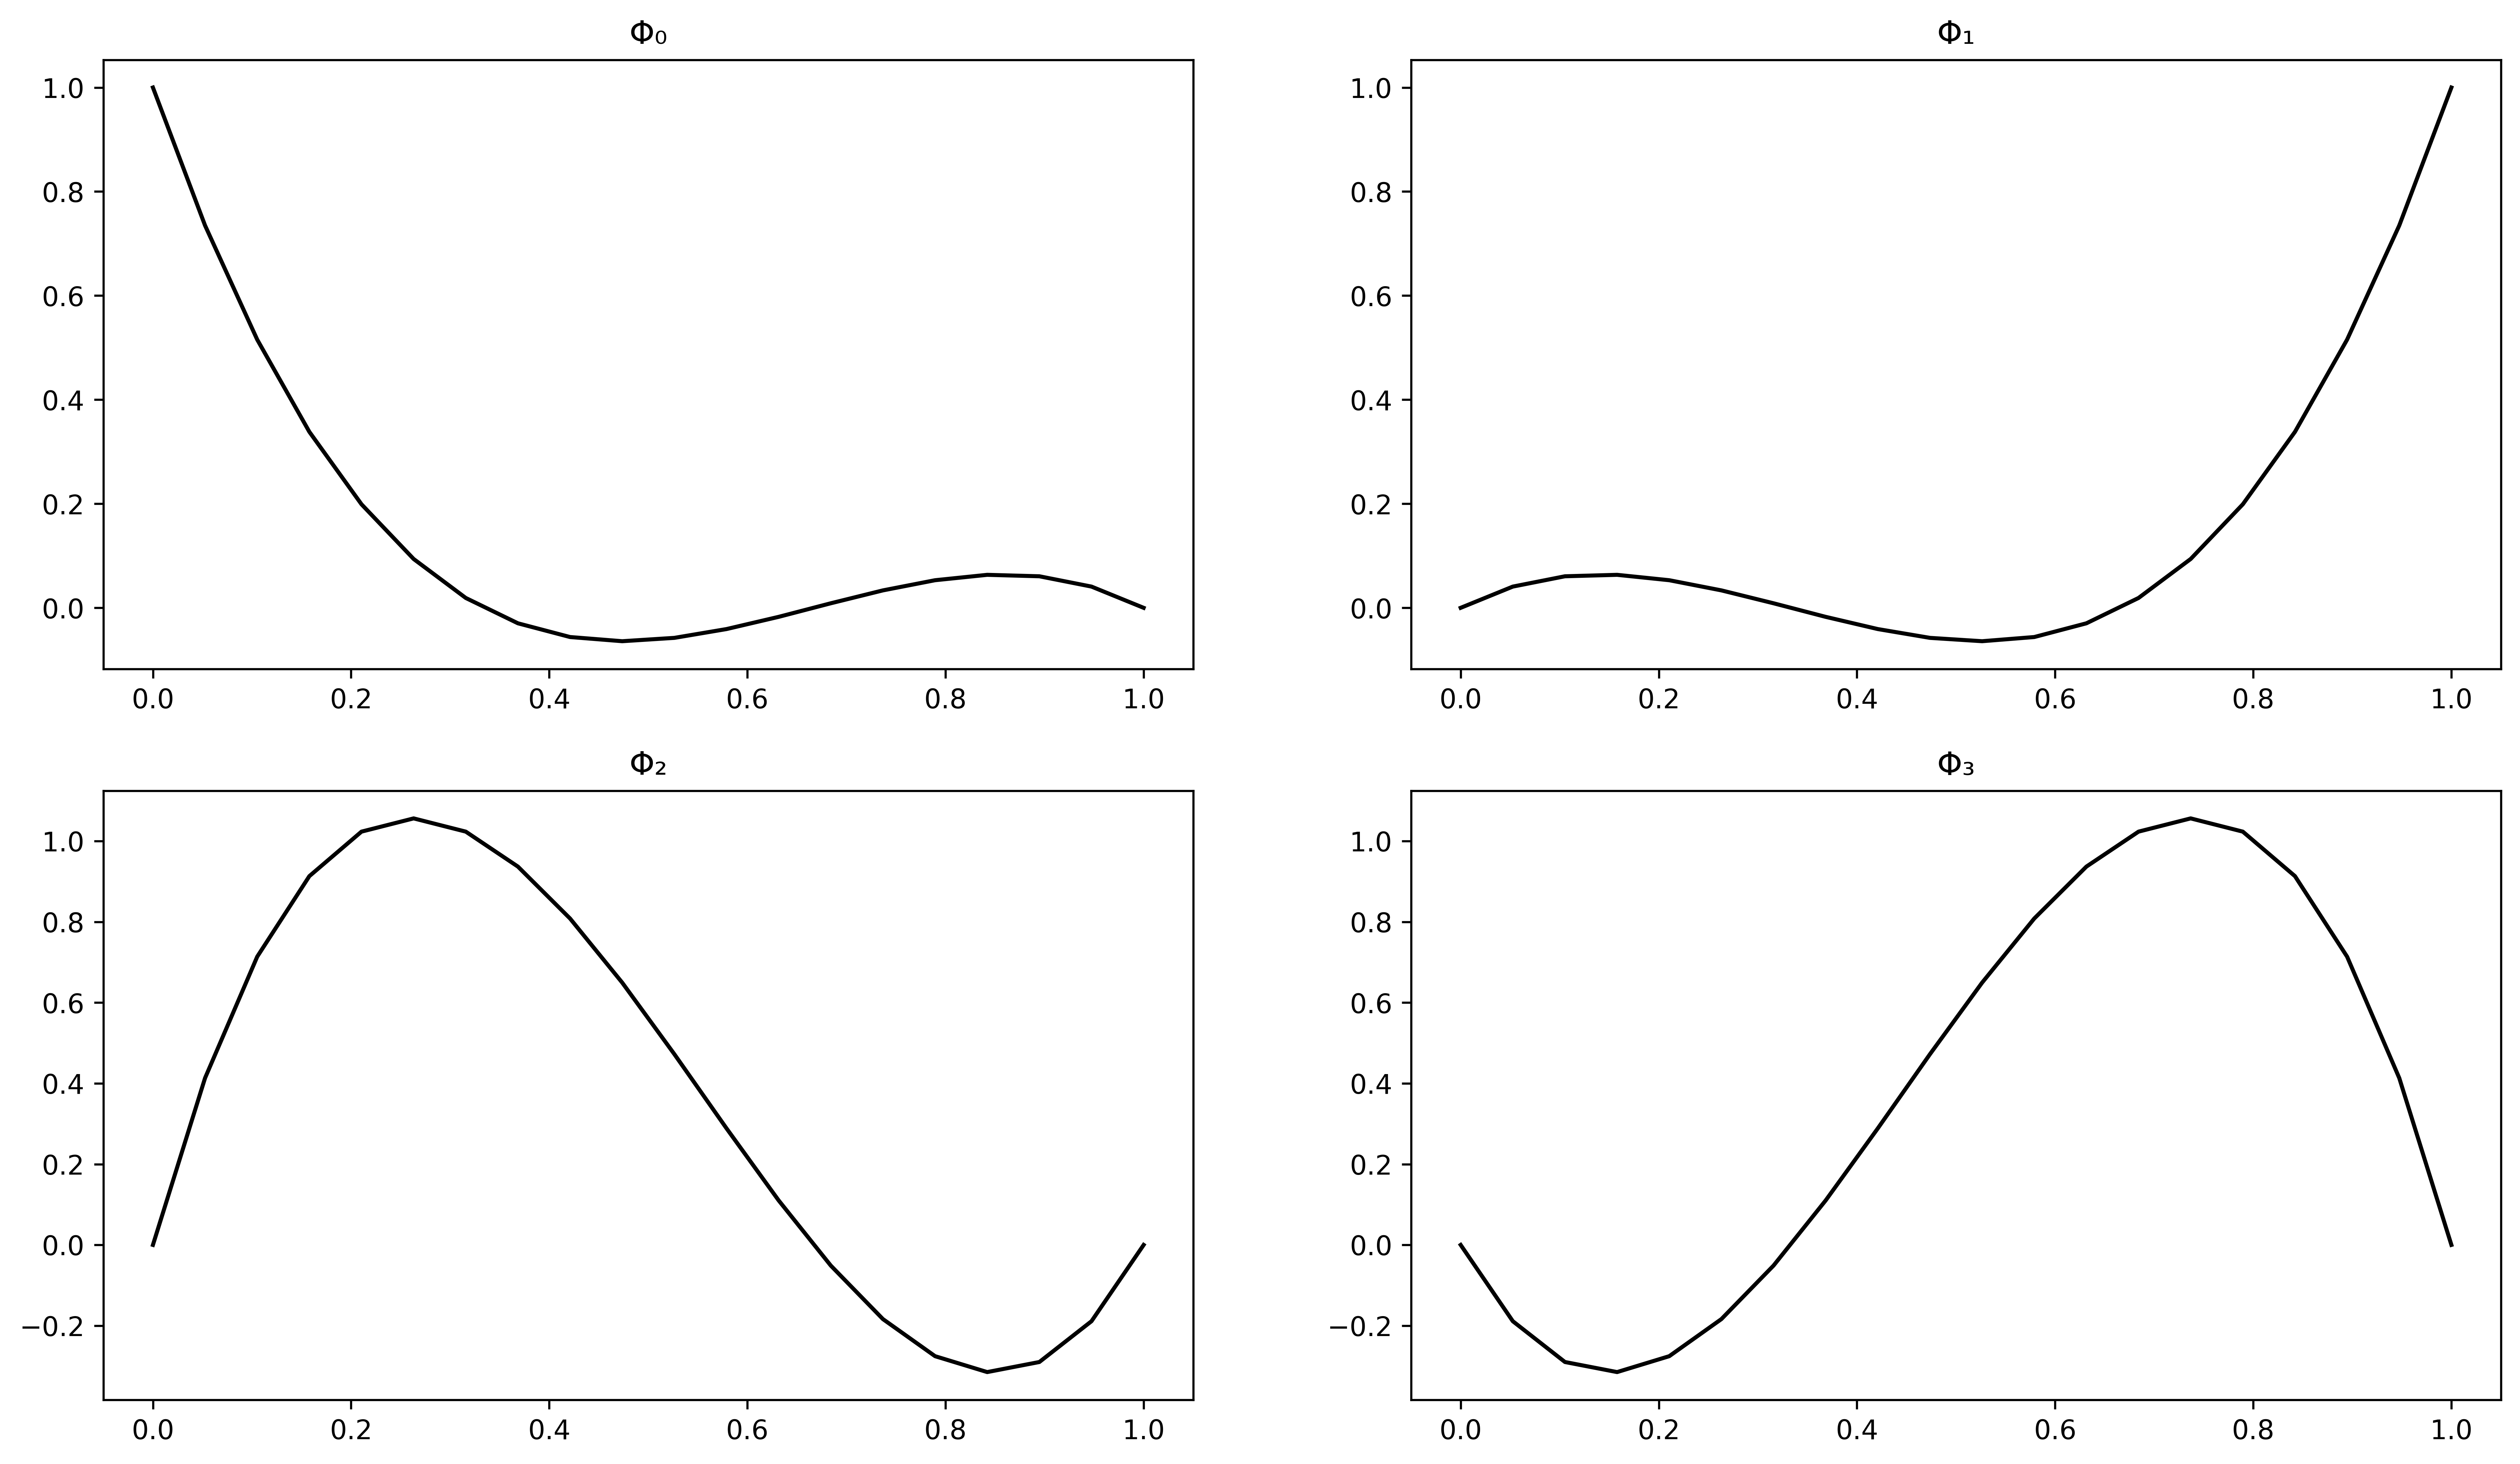
\includegraphics[width=.8\linewidth]{p3_mesh_basis}
    \caption{Polynomial of degree 3 on the unit interval}
  \end{subfigure}
  \caption{Polynomial basis on the 1d reference element}
  \label{fig:basis_1d}
\end{figure}


\begin{figure}
  \centering
  \begin{subfigure}{1.\textwidth}
    \centering
    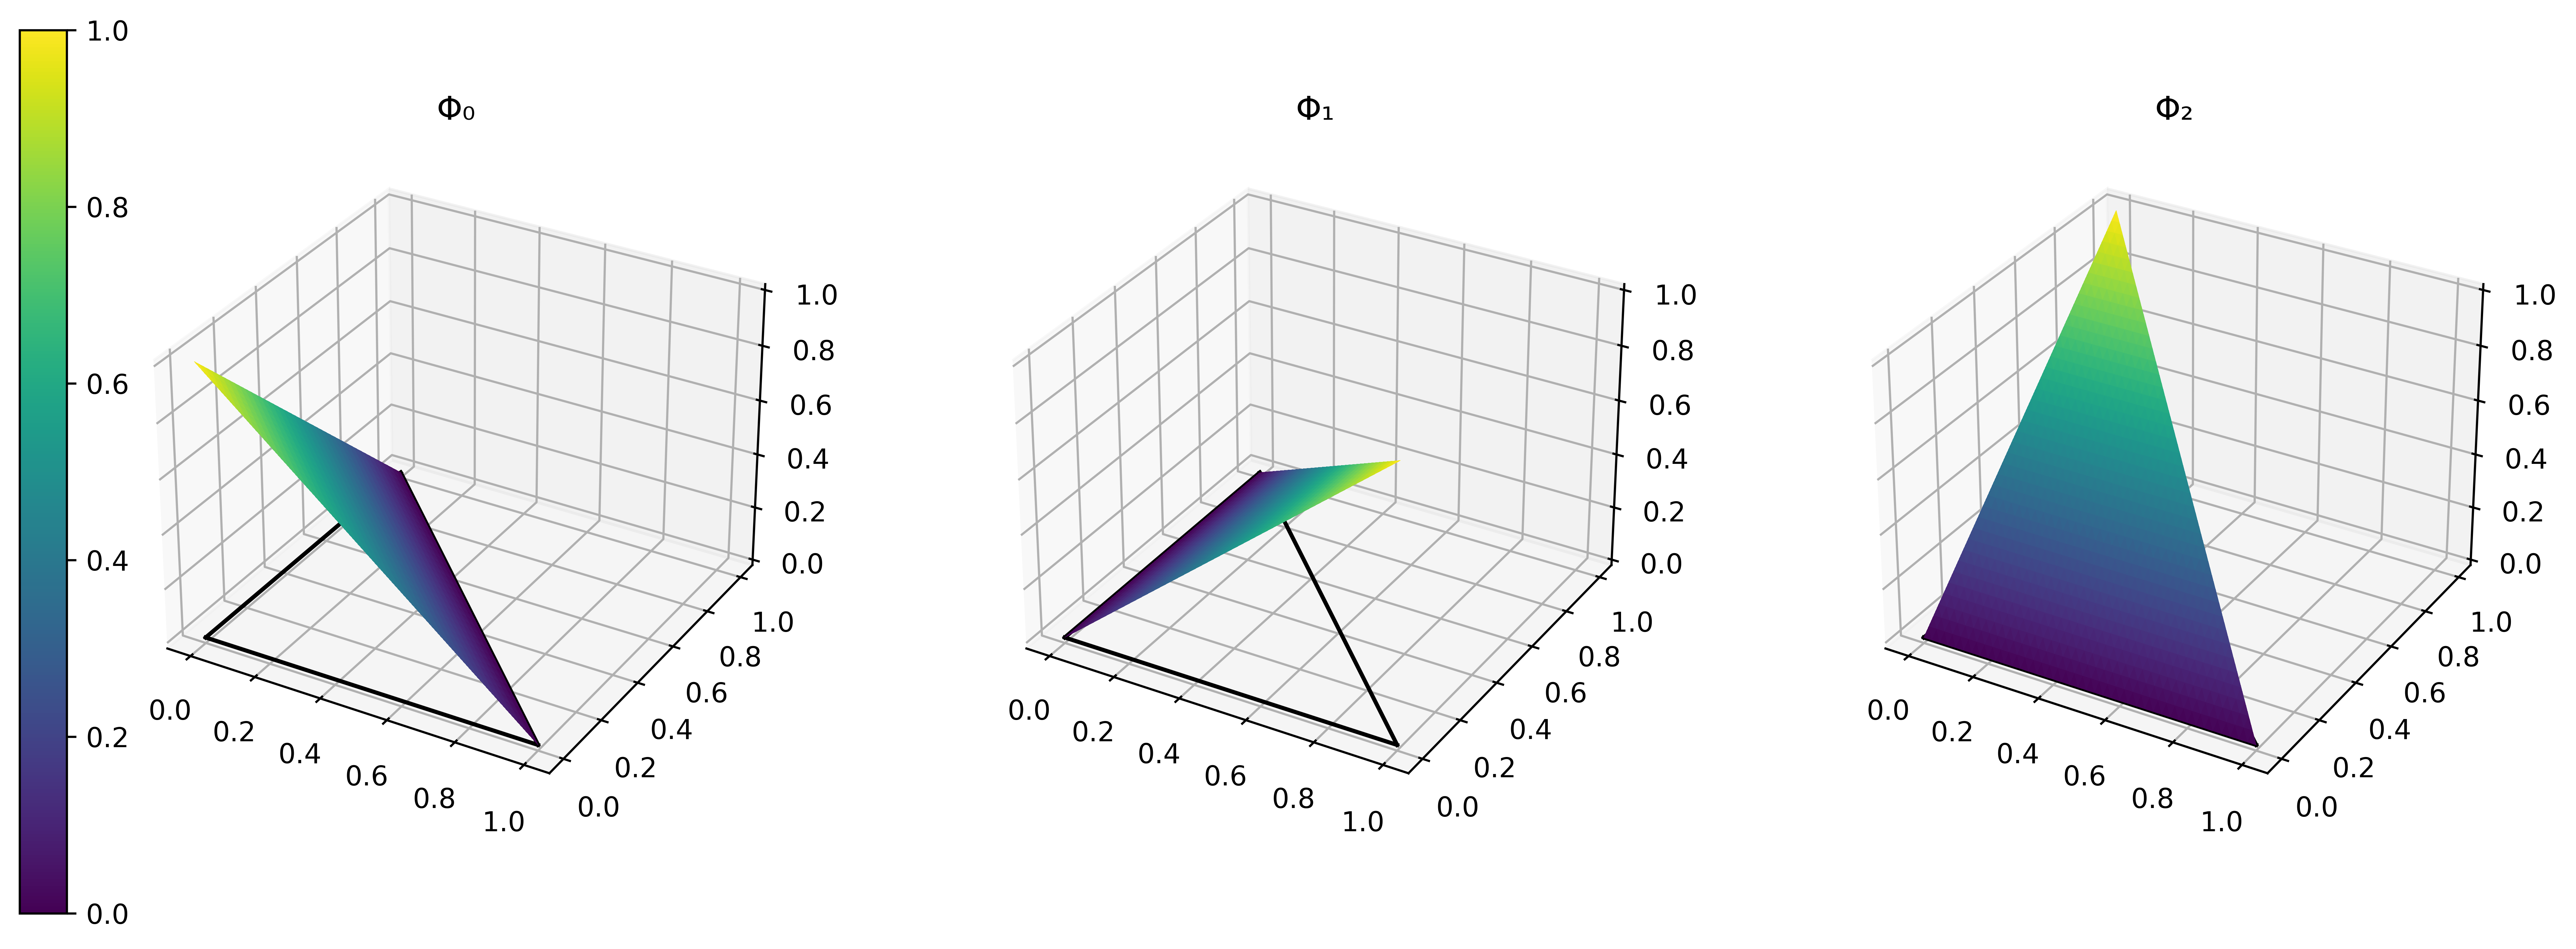
\includegraphics[width=.8\linewidth]{p1_2d_mesh_basis}
    \caption{Polynomial of degree 1 on the 2-unit-simplex}
  \end{subfigure}
  \begin{subfigure}{1.\textwidth}
    \centering
    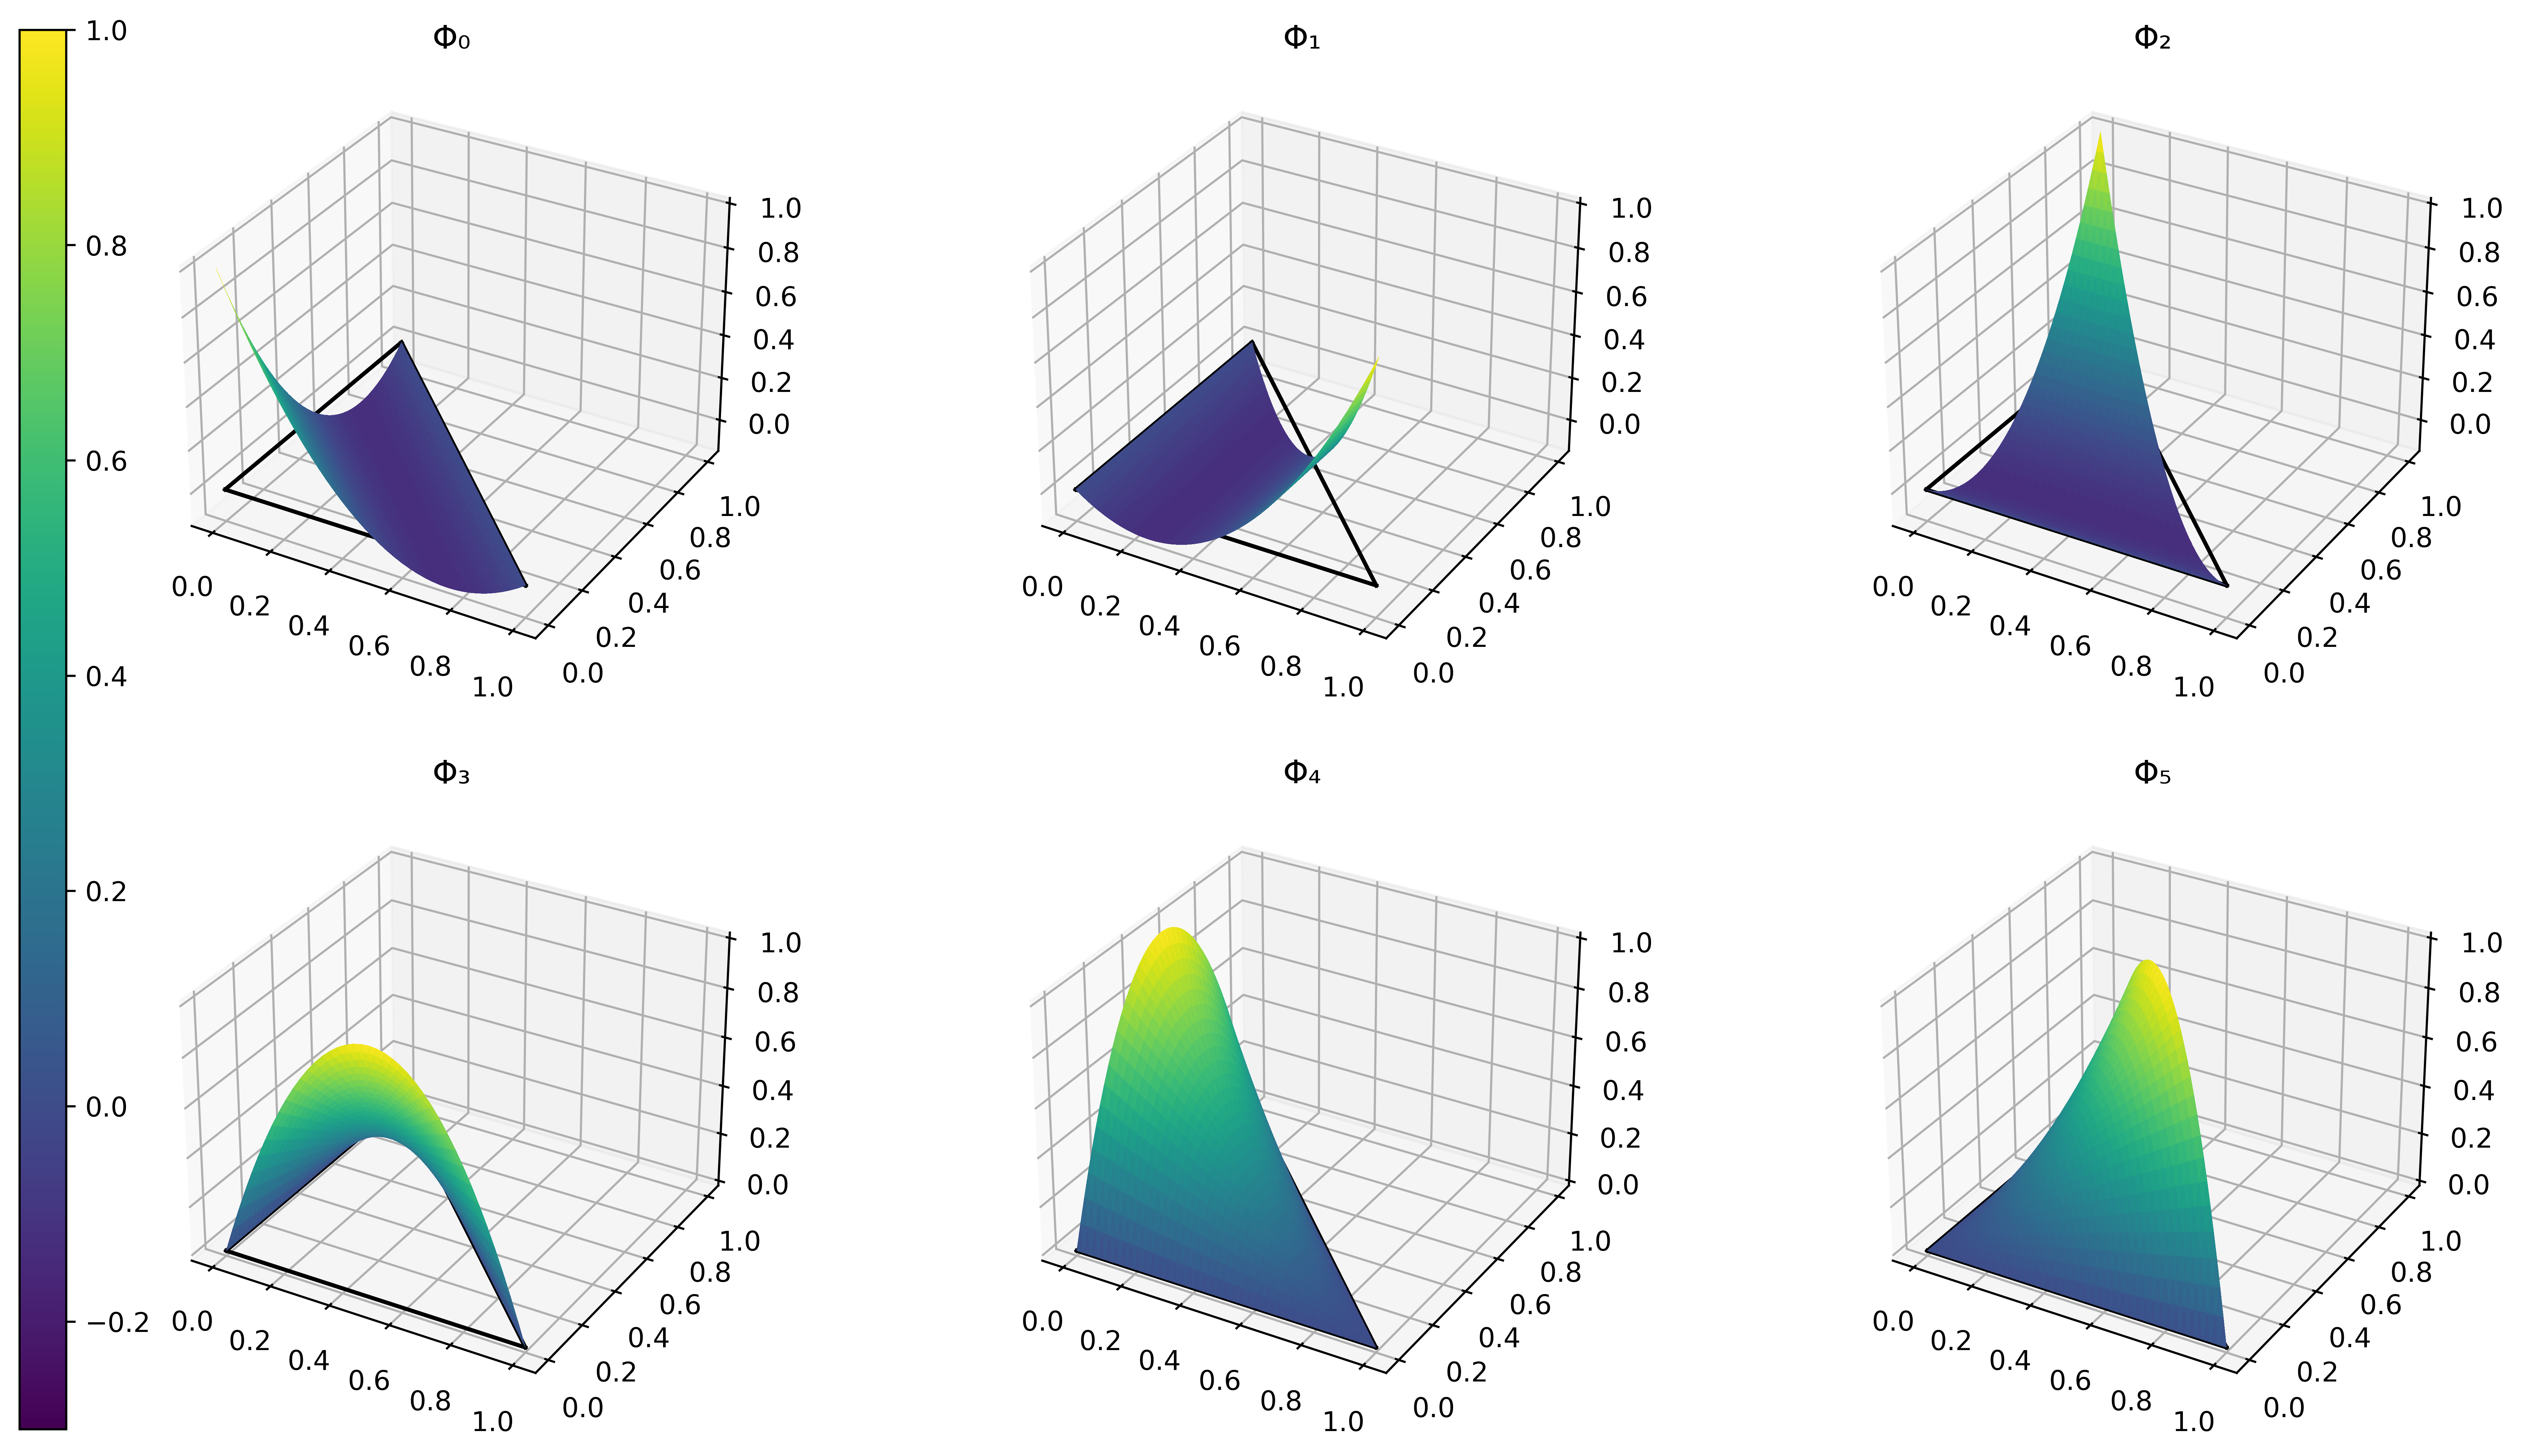
\includegraphics[width=.8\linewidth]{p2_2d_mesh_basis}
    \caption{Polynomial of degree 2 on the 2-unit-simplex}
  \end{subfigure}
  \caption{Polynomial basis on the 2d reference element}
  \label{fig:basis_2d}
\end{figure}


The following estimate for the convergence rates of $k^{\text{th}}$ order
elements has been established during the lecture:
\begin{equation}
  \lVert u - u_h \rVert_L^2 \lesssim h^{k'} \lVert u \rVert_{H^{k'+1}}
\end{equation}
Where $k' = \operatorname{min}\left(k,m\right)$ and $m$ is the largest integer s.t. $u \in H^{m+1}$.

By using Problem \ref{eq:} again, the parameter $a$ can be adjusted easily to
verify the above convergence rate for higher order elements.







\subsection*{Discretization}
The goal of the Finite Element Method is to approximate used Hilbert spaces by
finite dimensional subspaces. We will see that an approximation of $H^1(\Omega)$
suffices for the previously stated Poisson equation with Dirichlet or mixed
boundary conditions. For now, assume the problem in its general form:\\

Find $u \in V$ such that:
\begin{equation}
  a(u,v) = l(v), \quad \forall v \in V
\end{equation}

Given some Hilbert space $\left(V, \lVert \cdot \rVert_V\right)$, a functional
$l\in V'$ in the dual space of $V$ and a bilinear form $a: V \times V
\rightarrow \mathbb{R}$ which satisfies for all $u,v\in V$:
\begin{enumerate}
  \item $|a(u,v)| \leq M \lVert u \rVert_V \cdot \lVert v \rVert_V, \quad M > 0$
  \item $a(u,u) \geq \gamma \lVert u \rVert_V, \quad \gamma > 0$
\end{enumerate}


To construct a finite dimensional approximation of the above Hilbert space $V$
a sequence of subspaces $(V_n)_{n\in\mathbb{N}} \subset V$ can be constructed with:
$V_n = span(\Phi_1,\dotsb, \Phi_n)$ with some basis functions $\Phi_i$ and the
desired property $\lim\limits_{n\to \infty} V_n = V$.
The Lax-Milgram lemma now guarantees existence and uniqueness of a solution in
the finite dimensional subspace:
\begin{equation}
  a(u_n, v_n) = l(v_n), \quad \forall v_n \in V_n
\end{equation}

Or equivalently:
\begin{equation}
  a(u_n, \Phi_i) = l(\Phi_i), \quad \forall 1 \le i \le n
\end{equation}
where $u_n = \sum^n_1 \hat{u}_i\Phi_i$. This can be restated in terms of a
linear system:
$$Ax=b$$
where $A_{i,j} = a(\Phi_i, \Phi_j) \in \mathbb{R}^{n\times n}$,
$x = \left(\hat{u}_1, \dotsb, \hat{u}_n\right) \in \mathbb{R}^n$ and
$b = (l(\Phi_i), \dotsb, l(\Phi_n)) \in \mathbb{R}^n$.\\
At this point it has not been shown that solutions in the sequence of finite
dimensional subspaces will indeed converge to a solution in the infinite
dimensional space $V$. This will be done later, when convergence rates are
investigated. For now, assume that it indeed converges under reasonable
assumptions.

To obtain a sparse matrix $A$ and a fairly simple projection/interpolation
operator, isoparametric Lagrange elements on simplices are chosen. For now,
only linear finite elements will be considered. In section {\bf TODO} this will
be extended to arbitrary order polynomials.

As introduced in the lecture, a finite dimensional subspace $V_n \subset V$ is
obtained by approximating the underlying domain $\Omega$ by a conforming
subdivision into simplexes (mesh). Then local basis functions defined on a
reference simplex are mapped to global elements on the mesh.


\subsubsection{Reference Elements}
In $d$ spatial dimensions, the reference simplex is defined as:
$$T \coloneqq \left\{x \in \left[ 0,1 \right] ^d \, : \, \sum^d_{i=1} x_i \le 1\right\}$$
The space of $1^{\text{st}}$ order polynomials on $T$ has dimension $d+1$.
Thus, $d+1$ distinct points are needed to define a $1^{\text{st}}$ degree
polynomial space on $T$. Choosing the vertices of the simplex $T$ suffices in
this case and the local space can be defined as follows:
$$
\left\{ \phi_i: T \to \mathbb{R} \in \mathbb{P}_1 \, : \, \phi_i(x_j) = \delta_{ij},\quad 1 \le i,j \le d+1\right\}
$$
where the $x_j$ are the $d+1$ distinct vertices of the simplex. Fo $1$ and $2$
spatial dimensions, these spaces are visualized in fig {\bf TODO}.

\subsubsection*{Mapping to Global Elements in the Mesh}
For each simplex on the mesh, define $\Psi_k: T \to T_k$ where $T$ is the
reference simplex and $T_k$ is the $k^\text{th}$ simplex on the mesh.
$\Psi_k$ is fully determined by $\Psi_k(x_j)$ for all vertices of the simplex.

In the following, let $\Omega$ be a Lipschitz domain where its boundary
$\Gamma$ is approximated polygonally.






\begin{multicols}{2}

  \subsection*{Theory}
    The PDE in consideration is the stereotypical Poisson equation:
    \begin{equation}
      % \label{eq:poisson}
      - \nabla \cdot \left( \nabla u \right) = f \quad \text{on} \Omega
    \end{equation}

    Where solutions will be sought on the unit square $\Omega = \left[0,1\right]^2$.

    In this strong from \ref{eq:poisson} requires strong assumptions on $f$ and $\Omega$.
    In order to obtain a meaningful numerical method, these assumptions must be relaxed.
    This is done by multiplying both sides of the equation by test functions and integrating over the domain $\Omega$.
    For simplicity, assume $f = 0$ for now:
    \begin{equation}
      \label{eq:poisson_weak}
      - \int_\Omega \nabla \cdot \left(\nabla u\right) v \,dx = \int_\Omega fv \,dx
        \quad \forall v \in \mathcal{C}^\infty_0(\Omega)
    \end{equation}

    By applying Green's formula, it is obtained:
    \begin{equation}
      \int_\Omega \nabla u \cdot \nabla v \,dx - \int_\Gamma v \frac{\partial y}{\partial \nu} \,dS = \int_\Omega fv \,dx
        \quad \forall v \in \mathcal{C}^\infty_0(\Omega)
    \end{equation}

    Which can be further simplified, because $v = 0$ on $\Gamma$.
    Resulting in weak formulation of the Poisson problem with homogeneous Dirichlet boundary condition:
    \begin{equation}
      \underbrace{\int_\Omega \nabla u \cdot \nabla v \,dx}_{\coloneqq a(u,v)} = \underbrace{\int_\Omega fv \,dx}_{\coloneqq l(f)}
        \quad \forall v \in \mathcal{C}^\infty_0(\Omega)
    \end{equation}

    Where $\mathcal{C}^\infty_0(\Omega)$ is the space of smooth test functions vanishing at the boundary.
    As mentioned in the lecture, $\mathcal{C}^\infty_0(\Omega)$ is dense in $H^1_0(\Omega)$ w.r.t. the $H^1$ norm.
    Since both sides of \ref{eq:poisson_weak} are continuous w.r.t. $v$, \ref{eq:poisson_weak} also holds for all $v \in H^1_0(\Omega)$.

    Since, both, the above defined bilinear form $a$ is bounded and coercive, as well as $l \in H^{-1}_0$,
    Lax-Milgram guarantees existence and uniqueness of a solution.

    Lax-Milgram additionally guarantees that $u$ is the unique minimizer of
    \begin{equation}
      \min_{y \in H^1_0} \frac{1}{2}a(y,y) - l(y)
    \end{equation}
    This can later be used to implement boundary conditions.

  \subsubsection*{Boundary Conditions}
    \begin{theorem}
     The Poisson equation with Dirichlet and Neumann boundary conditions:
      \begin{align*}
        -\nabla \cdot \left( \nabla u \right) &= f  \text{ in } \Omega\\
        u &= g \text{ on } \Gamma_0\\
        \frac{\partial u}{\partial \nu} &= h \text{ on } \Gamma_1
      \end{align*}
      with $f \in L^2(\Omega)$, $g \in L^2(\Gamma_0)$, $h \in L^2(\Gamma_1)$ and $\int_{\Gamma_0}\,dx > 0$.
      Has a weak solution $u \in H^1(\Omega)$.

      \begin{proof}
        Obtain the weak formulation as usual:
        \begin{equation*}
          \label{eq:poisson_weak_boundaries}
          \int_\Omega \nabla u \cdot \nabla v \,dx - \int_{\Gamma_0} v \frac{\partial u}{\partial \mu} \,dx =
            \int_\Omega fv\,dx + \int_{\Gamma_1} vh\,dx
        \end{equation*}

        Furthermore define the Hilbert spaces:
        \begin{align*}
          V_0 &= \left\{ v \in H^1(\Omega)\, :\, v\vert_{\Gamma_0} = 0 \text{ a.e. on } \Gamma_0 \right\}\\
          V_g &= \left\{ v \in H^1(\Omega)\, :\, v\vert_{\Gamma_0} = g \text{ a.e. on } \Gamma_0 \right\}
        \end{align*}

        And define the bilinear form $a$ and linear functional $l$ as follows:
        \begin{align*}
          a(u,v) &= \int_\Omega \nabla u \cdot \nabla v \,dx\\
          l(v)   &= \int_{\Gamma_1} hv \,dx + \int_\Omega fv\,dx
        \end{align*}

        Lax-Milgram guarantees existence of a unique solution to:
        \begin{equation*}
          a(u,v) = l(v) \quad \forall v \in V_0
        \end{equation*}
        If $\int_{\Gamma_0}dx >0$

        Now choose an arbitrary $\hat{g}\in V_g$ and solve:
        \begin{equation*}
          a(\hat{u},v) = l(v) - a(\hat{g},v) \quad \forall v \in V_0
        \end{equation*}

        The solution to \ref{eq:poisson_weak_boundaries} is obtained by:
        $$u = \hat{u} + \hat{g} \in V_g$$

      \end{proof}

    \end{theorem}

  \subsection*{Grid Generation}

\end{multicols}

\end{document}
